
\documentclass[12pt,a4paper,twoside]{book}
\usepackage{subfigure}
\usepackage{amsmath}
\usepackage{mathrsfs}
\usepackage{wasysym}
\usepackage{lineno}
\usepackage{authblk}
\usepackage{rotating}
\usepackage{rotfloat}
%\usepackage{color}
\usepackage{multirow}
\usepackage{xspace}
\usepackage{rotating}
\usepackage{hyperref}
\usepackage{enumitem}
\usepackage{cite}
%\usepackage[margin=1.in]{geometry}
\usepackage{geometry}
%\usepackage[sorting=none]{biblatex}
\hypersetup{pdfborder = 0 0 0}
%\usepackage[titletoc]{appendix}
%\usepackage{graphicx}
%\usepackage{caption}
%\usepackage{subcaption}

% \usepackage{feynarts} 
\listfiles
%%%%%%%%%%%%%%%%%%%%%%%%%%%%%%%%%%%%%%%%%%%%%%%%%%%%%%%%%%%%%%%%%%%%%%%%%%%%%%%
% This is where the document really begins
%%%%%%%%%%%%%%%%%%%%%%%%%%%%%%%%%%%%%%%%%%%%%%%%%%%%%%%%%%%%%%%%%%%%%%%%%%%%%%%

% Shorthand for \phantom to use in tables
\newcommand{\pho}{\phantom{0}}
\newcommand{\bslash}{\ensuremath{\backslash}}
\newcommand{\BibTeX}{{\sc Bib\TeX}}

% Org def
\newcommand{\mT}{\ensuremath{m_{\mathrm{T}}}\xspace}
%\def\mT{\ensuremath{M_{\mathrm{T}}}}
\def\rqcd{\ensuremath{r_{\mathrm{QCD}}}\xspace}
\def\kqcd{\ensuremath{k_{\mathrm{QCD}}}}
\def\rwjets{\ensuremath{r_{W\mathrm{+jets}}}}
\def\kwjets{\ensuremath{k_{W\mathrm{+jets}}}}
\def\rztautau{\ensuremath{r_{Z\rightarrow\tau\tau}}}
\def\rother{\ensuremath{r_{\mathrm{other}}}}
\def\kztautau{\ensuremath{k_{Z\rightarrow\tau\tau}}}
\def\kother{\ensuremath{k_{\mathrm{other}}}\xspace}
\def\mVis{\ensuremath{M_{\tau\tau}^{\mathrm{visible}}}\xspace}
\def\nOSmVis{\ensuremath{n_{\mathrm{OS}}(m_{\mathrm{vis}})}}
\def\nOSqcd{\ensuremath{n_{\mathrm{OS}}^{\mathrm{QCD}}}}
\def\nOSwjets{\ensuremath{n_{\mathrm{OS}}^{W\mathrm{+jets}}}}
\def\nOSztautau{\ensuremath{n_{\mathrm{OS}}^{Z\rightarrow\tau\tau}}}
\def\nOSother{\ensuremath{n_{\mathrm{OS}}^{\mathrm{other}}}}
\def\nSSall{\ensuremath{n_{\mathrm{SS}}^{\mathrm{all}}}}
\def\nSSqcd{\ensuremath{n_{\mathrm{SS}}^{\mathrm{QCD}}}}
\def\nSSwjets{\ensuremath{n_{\mathrm{SS}}^{W\mathrm{+jets}}}}
\def\nSSztautau{\ensuremath{n_{\mathrm{SS}^{Z\rightarrow\tau\tau}}}}
\def\nSSother{\ensuremath{n_{\mathrm{SS}}^{\mathrm{other}}}}
\def\nSSallmVis{\ensuremath{n_{\mathrm{SS}}^{\mathrm{all}}(m_{\mathrm{vis}})}}
\def\nSSqcdmVis{\ensuremath{n_{\mathrm{SS}}^{\mathrm{QCD}}(m_{\mathrm{vis}})}}
\def\nSSwjetsmVis{\ensuremath{n_{\mathrm{SS}}^{W\mathrm{+jets}}(m_{\mathrm{vis}})}}
\def\nOSztautaumVis{\ensuremath{n_{\mathrm{OS}}^{Z\rightarrow\tau\tau}(m_{\mathrm{vis}})}}
\def\nSSztautaumVis{\ensuremath{n_{\mathrm{SS}}^{Z\rightarrow\tau\tau}(m_{\mathrm{vis}})}}
\def\nOSothermVis{\ensuremath{n_{\mathrm{OS}}^{\mathrm{other}}(m_{\mathrm{vis}})}}
\def\nSSothermVis{\ensuremath{n_{\mathrm{SS}}^{\mathrm{other}}(m_{\mathrm{vis}})}}
\def\ttbar{\ensuremath{t\bar{t}}\xspace}
\def\PT{\ensuremath{p_{T}}\xspace}
\def\pt{\ensuremath{p_{T}}\xspace}
\def\GeV{\ensuremath{\text{GeV}}\xspace}
\def\Zee{\ensuremath{Z\rightarrow ee}\xspace}
\def\Zmumu{\ensuremath{Z\rightarrow \mu\mu}\xspace}
\def\Ztautau{\ensuremath{Z/\gamma^*\rightarrow \tau\tau}\xspace}
\def\Ztt{\ensuremath{Z\rightarrow \tau\tau}\xspace}
\def\Wlnu{\ensuremath{W\rightarrow \ell \nu}\xspace}
\def\Zll{\ensuremath{Z\rightarrow \ell \ell}\xspace}
\def\nqcd{\ensuremath{n^{QCD}}\xspace}
\def\rqcd{\ensuremath{R_{QCD}}\xspace}
\def\ToTauTauLepHad{\ensuremath{\rightarrow\tau\tau\to \ell\tau_{had}}\xspace}
\def\ToTauTauLepLep{\ensuremath{\rightarrow\tau\tau\to \tau_{\ell}\tau_{\ell}}\xspace}
\def\MET{\ensuremath{E_{T}^{miss}}\xspace}
\def\met{\ensuremath{E_{T}^{miss}}\xspace}
\def\Ht{\ensuremath{H_{T}}\xspace}
\def\etcone{\ensuremath{E_{T}(\mathrm{cone})} }
\def\ptcone{\ensuremath{p_{T}(\mathrm{cone})} }
\def\SumLtMET{\ensuremath{p_{T\mu} + p_{Te}+\met} }
\def\mmc{\ensuremath{m_{\tau\tau}^{MMC}} }
\def\MMC{\ensuremath{MMC_{mass}} }
\def\mA{\ensuremath{M_{A}}}
\def\mh{\ensuremath{M_{h}}}
\def\mH{\ensuremath{M_{H}}}
\def\mHp{\ensuremath{M_{H^\pm}}}
\def\ifb{\ensuremath{fb^{-1}} }

\linespread{1.3}
\begin{document}
\tableofcontents

%\clearpage
%%%%%%%%%%%%%%%%%%%%%%%%%%%%%%%%%%%%%%%%%%%%%%%%%%%%%%%%%%%%%%%%%%%%%%%%%%%%%%%
%%									     %%		
%%			TRAMA DELLO PSYCHO-TRILLER			     %%
%%									     %%	
%%%%%%%%%%%%%%%%%%%%%%%%%%%%%%%%%%%%%%%%%%%%%%%%%%%%%%%%%%%%%%%%%%%%%%%%%%%%%%%
%%%%%%%%%%%%%%%%%%%%%%%%%%%%%%%%%%%%%%%%%%%%%%%%%%%%%%%%%%%%%%%%%%%%%%%%%%%%%%%
%%  Elementi importanti:                                                     
%%	Statistica ; Descrizione degli oggetti come ele, mu ecc..	     
%%	Data MC sample ; Embedding  ; MMC ;  Corrections	
%%
%%  Struttura Analisi part:
%%	*) motivazioni ; 											| Sezione riguardante quello che ti proponi di fare
%%	*) Strategia: Quale e' la nostra Hypotesis 0, vogliamo fare un test di ipotesi (prima parte Stat).. 	|
%%	   punti chiave che differenziano MSSM higgs da SM e la strategia per sfruttarne i vantaggi (b-tag veto)|
%%	   Selezioni spiegando bene le motivazioni di ciascuna	(full preselections in appendice)		|
%%         MMC													|
%%
%%	*) Background Modeling: Impatto con la realta' delle cose (data driven bkg estimation del quale non ci sarebbe bisogno se tutto fosse perfetto)   | come lo
%%	   quindi si presenta un Problema e ne si da' la soluzione (bkg estimation)									  | Fai
%%	   Data MC sample, Embedding 															  |
%%	*) determinazione sys, che pero' possono essere splittate in due ---> una in tesi l'altra in appendix (che non ce ne frega una sega dei dettagli) |
%%	
%%	*) Risultati:  parte aggiuntiva su stat. e limiti.
%%
%%	
%%
%%  Struttura resto:	
%%	*) Theory   
%%	*) Atlas detector + descrizione degli oggetti + performance + corrections
%%	*) Trackjets
%%
%%  Try to not suicide...	
%%
%%
%%
%%
%%
%%
%%
%%
%%
%%
%%

%Theory
%\chapter{The Higgs Bosons and the MSSM}
This chapter is devoted to introduce the the Minimal Supersymmetric 
extension of the Standard Model (MSSM) whit focus on  its Higgs sector.
In section... introduction is given based on~\cite{Altarelli}, 


\clearpage

\section{The Standard Model of Particle Physics and its Limitations}
\subsection{Overview of the SM}
The Standard Model (SM) of particle physics is a theory aimed to describe and quantitatively predict
the phenomenology of foundamental interaction. At ``microscopic''  level all the phenomenology of matter and 
radiation can be understood in terms of three classes of foundamental interactions, which are the strong, the electromagnetic
and the weak interactions, the gravitational force is instead negligible in atomic and nuclear physics (quantum effects in gravity are
expected to become important at energies corresponding to the Planck mass $E \sim M_{planck} c^2 \sim 10^{19}$ GeV).
All these interactions (with the exception of gravity) are described by a local relativistic quantum field theory.
To each particle, described as pointlike, is associated a field with suitable
(depending on the particle spin) transformation properties under the Lorentz group (the
relativistic space-time coordinate transformations). The description
of all these particle interactions is based on a common principle: ``gauge'' invariance. A
gauge symmetry is invariance under transformations that rotate the basic internal degrees of freedom but
 with rotation angles that depend on the space-time point.

The SM is a gauge field theory based on the symmetry group $SU(3)_c \otimes SU(2)_L \otimes U(1)_Y$. This group has $8+3+1=12$
generators with a non trivial commutator algebra. The electromagnetic and weak interactions (EW) are described \cite{} by the 
$SU(2)_L \otimes U(1)_Y$ symmetry group, while the $ SU(3)_c$ is the colour group of the theory of strong interactions (QCD)~\cite{}.
To each generator of the symmetry group is associated a vector boson which act as mediator of the correspondig interactions.
Eight gluons are associated to the $ SU(3)_c$ colour generators, while for $SU(2)_L \otimes U(1)_Y$ there are four gauge bosons $W^{\pm}$,
$Z^0$ and $\gamma$. Of these, only the gluons and the photon are massless since the symmetry induced by the other three generators is
spontaneusly broken. In the SM the spontaneus symmetry breacking is realized by the Higgs mechanism~\cite{}, the Higgs particle has 
been recently found at the LHC with $m_H \sim 125$ GeV \cite{} representing one of the major mailstone of particle physics.
The Higgs boson acts as mediator of a new class of interactions that, at tree level, are coupled in proportion to the particle masses.

The fermionic (all of spin 1/2) matter fields of the SM are quarks and leptons. 
Quarks  are subject to all SM interactions, each type of quark is a colour triplet and carries 
electroweak charges, in particular electric charges $+2/3$ for up-type quarks and $-1/3$
for down-type quarks.  Leptons are colourless
but have electroweak charges, in particular electric charges $-1$ for charged leptons $e$, $\mu$ and $\tau$ (opposite sign charge 
is intended for respective anti-particle)  and charge 0 for neutrinos $\nu_e$, $\nu_{\mu}$ and $\nu_{\tau}$.
Qarks and leptons are grouped in three  ``generations'' with equal quantum numbers but different masses.

\subsection{Precision Test and Limitation of the SM}

Precision tests of the SM has been performed over a wide range of energies in experiment in the last several decades,
Precision tests~\cite{precisiontest} of the standard electroweak theory performed at LEP, SLC and Tevatron~\cite{smtest}, 
has confirmed the couplings of quark and leptons to the weak gauge bosons $W^{\pm}$  and $Z$ are indeed
precisely those prescribed by the gauge symmetry. The accuracy of a few per-mille for these
tests implies that, not only the tree level, but also the structure of quantum corrections has
been verified. Several other experimental results~\cite{pdg} rare decays and the anomalus magnetic moment of the muon
provide a test for low-energies of the standard model.

%However 
%In spite of this success, the conceptual situation with the
%standard model is unsatisfactory for quite a few deficiencies:
%– the smallness of the electroweak scale v ∼ 246GeV << MPl (the ‘hierarchy problem’);
%– the large number of free parameters (gauge couplings,
%vacuum expectation value, MH, fermion masses,
%CKM matrix elements), which are not predicted but have
%to be taken from experiments;
%– the pattern that occurs in the arrangement of the
%fermion masses;
%– the missing way to connect to gravity.
%
%-Dark matter
%
%-neutrino masses

 
\section{The Minimal Supersymmetric Standard Model}
\subsection{Introduction}
Supersymmetry (SUSY) was first introduced since it offer a natural way to solve the hierarchy problem....\cite{}
This is achieved by introducing a symmetry transformation that relates bosons with fermions. The SUSY generators $\mathcal{Q}$ 
transforms fermion into bosons and vice versa:
\begin{equation}
\mathcal{Q}|\text{Fermion}\rangle = |\text{Boson}\rangle, ~ ~ ~ \mathcal{Q}|\text{Boson}\rangle = |\text{Fermion}\rangle
\end{equation}
This is suggesting that in a supersymmetric extesion of the SM \cite{page7Martins} each of the known foundamental particles 
is in either a chiral or gauge ``supermultiplet'' and must have a superpartner with spin differing by 1/2 unit.
Fermions since the left-handed and right-handed component transform differently under gauge transformations also their superpartner 
should maintain this property, the name of the superpartner of the quarks and leptons are made by adding an ``s'' to the SM name, standing for scalar.
Accordingly, the gauge bosons related to the generator of the group $SU(3)_c \otimes SU(2)_L \otimes U(1)_Y$ should also have a spin 1/2 partner,
whose name will be made by adding a ``ino'' at the end of the SM name. The symbol of superpartners is defined by adding a ($\tilde{ ~ }$) to the SM symbol.

The  Minimal Supersymmetric extension of the Standard Model  (MSSM)~\cite{page11Djuadi}, is defined by requiring the minimal gauge group (i.e., the SM one)
and the minimal particle content: three generation of fermions (without right-handed neutrinos), gauge bosons and two Higgs doublet, 
each with its superpartners. Tables~\ref{tab:chiralsup} and~\ref{tab:gaugesup} summarize chiral and gauge supermultiplets in the MSSM.
This guys will mix to form neutralino and chargino....
\begin{table}
\begin{center}
\renewcommand{\arraystretch}{1.5}
\begin{tabular}{c|ccc}
\hline%\noalign{\smallskip}
Names 			&Supermultiplets	&	Spin 1/2  		& Spin 0 \\%[0.1cm]
\hline%\noalign{\smallskip}		
quark, squarks		& $Q$ 			&	$(u_L ~ d_L)$		& $( \tilde{u}_L ~ \tilde{d}_L)$ \\%[0.1cm]
($\times$ 3 families)	& $\bar{u}$		& 	$u_R^{\dagger}$ 	& $\tilde{u}_R^*$ \\%[0.1cm]
			& $\bar{d}$		& 	$d_R^{\dagger}$ 	& $\tilde{d}_R^*$ \\%[0.1cm]
\hline%\noalign{\smallskip}
leptons, sleptons	& $L$			&   	$(\nu ~ e_L)$ 		&  $( \tilde{\nu} ~ \tilde{e}_L)$\\%[0.1cm]
($\times$ 3 families)	& $\bar{e}$		&	$e_R^{\dagger}$         & $\tilde{e}_R^*$ \\%[0.1cm]
\hline%\noalign{\smallskip}
higgsinos, Higgs	& $H_1$			&	$( \tilde{H}_1^0 ~ \tilde{H}_1^-)$  &	$( H_1^0 ~ H_1^-)$ \\%[0.1cm]	 
			& $H_1$			&	$( \tilde{H}_2^+ ~ \tilde{H}_2^0)$  &	$( H_2^+ ~ H_2^0)$ \\%[0.1cm]	 
\hline
\end{tabular}
\caption{This table is based on~\cite{SusyPrimer} and summarize the chiral supermultiplets in the Minimal Supersymmetric Standard Model. The spin-0 fields are complex scalars
	and the spin-1/2 are left-handed two-component Weyl fermions.}
\label{tab:chiralsup}
\end{center}
\end{table}

\begin{table}
\begin{center}
\renewcommand{\arraystretch}{1.5}
\begin{tabular}{c|cc}
Names			& Spin 1 		&	Spin 1/2 \\
\hline
gluon, gluino		& $g$			& $\tilde{g}$	\\
W bosons, winos		& $W^{\pm}$ $W^0$	& $\tilde{W}^{\pm}$ $\tilde{W}^0$ \\
B boson, bino		& $B^0$			& $\tilde{B}^0$ \\
\hline
\end{tabular}
\caption{This table is based on~\cite{SusyPrimer} and summarize the gauge supermultiplets in the Minimal Supersymmetric Standard Model.}
\label{tab:gaugesup}
\end{center}
\end{table}

\subsubsection{$R$-parity conservation}
The MSSM also requires a discrete and multiplicative symmetry called $R$-parity~\cite{djuadi12}, this symmetry assures barion and lepton number 
conservation and it is defined as follows:
\begin{equation}
R_p = (-1)^{2s+3B=L}
\end{equation}
where $L$ and $B$ are lepton and barion numbers and $s$ stands for the spin quantum number. R-parity quantum numbers has value $+1$ for ordinary
SM particles and $-1$ for their superpartners. This symmetry was first introduced to overcome the problem of instability of the proton,
lepton and barion number violation leads, in many cases, 
to unstable proton with life-time shorter than the experimental lower limit. However the conservation of $R$-parity has also other important 
fenomenological consequences, SUSY particle are always produced in pairs and in their decay there is always an odd number of SUSY particle, 
and the lightest SUSY particle is stable, providing a good candidate for dark matter.


\subsubsection{The Soft SUSY Breaking}
In case the Supersymmetry is an exact symmetry of nature, the bosonic fields and the corrispective fermion fields should have the same mass 
and quantum numbers, except for the spin. However, the particle spectrum of SUSY has not yet been observed, suggesting that these particle
 should have an higher mass than their SM superpartners. 
To achieve SUSY-breaking in a way which does not reintroduce the quadratic divergences to the Higgs mass squared, a so called ``soft-SUSY-breaking''
term is introduced~\cite{djuadipage5orBetterPage12}, this term explicitly break SUSY introducing ad hoc the mass terms for Higgs, gauginos and
sferions, furthermore  trilinear coupling terms between sfermions and Higgs bosons are introduced. In general, if intergenerational mixing and 
complex phases are allowed, the soft-SUSY-breaking terms will introduce a huge number of unknown parameters $\mathcal{O}(100)$~\cite{djuadiPage5}.
However, in absence of phases and  mixing, and if obey to a set of boundary conditions~\cite{djuadi5}, only few new parameters are introduced.




\subsection{The Higgs Sector in the MSSM }
In the MSSM two doublets of complex scalar field of opposite hypercharge are required to break the electroweak symmetry, 
this requirement is motivated by the needs to generate  masses separately to isospin up-type fermion and down-type fermions~\cite{djouadiP21}
and to cancel chiral anomalies that otherwise would spoil the renormalizability of the theory~\cite{djouadiP21}. The two Higgs doublet then are:
\begin{equation}
H_1 = \binom{H_1^0}{H_1^-} ~ ~ \text{with } Y_{H_1} = -1, \quad \quad H_2 = \binom{H_2^+}{H_2^0} ~ ~ \text{with } Y_{H_2} = +1  
\end{equation}
In analogy with the SM, a similar Higgs mechanism is employed in the MSSM~\cite{djuadiP22},  requiring that the minimum 
of the Higgs potential breaks $SU(2)_L \otimes U(1)_Y$ group while preserving the electromagnetic symmetry $U(1)_Q$.
the  to break electroweak symmetry. The neutral components of the 
two Higgs field acquire vacuum expectation values:
\begin{equation}
\langle H_1^0 \rangle = \frac{v_1}{\sqrt{2}}, \quad \quad \quad  \langle H_2^0 \rangle = \frac{v_2}{\sqrt{2}}
\end{equation}
Three of the original eight degrees of freedom of the scalar fields are absorbed by the $W^{\pm}$ and $Z$ bosons, building their lomgitudinal
polarizations and acquire masses. The remaning degrees of freedom correspond to five scalar Higgs bosons: two CP-even and neutral $h$ and $H$, 
a neutral pseudoscalar boson $A$ and a pair of charged bosons $H^{\pm}$. At tree level, besides the masses of these particle, two additional parameter
define the system: the mixing angle in the neutral CP-even sector $\alpha$ and the ratio between the two vacuum expectation value $\tan \beta = v_1/v_2$.
However, the supersymmetric structure of the theory impose strong constraint on the Higgs spectrum, out of the six parameters which describe 
the MSSM Higgs sector, $M_h$, $M_H$, $M_A$, $M_{H^\pm}$, $\beta$ and $\alpha$, only two  are actually independent at tree level, a common choice 
is $\tan \beta$ and $M_A$. At tree level these relation impose a strong hierarchical structure on the mass spectrum: the $h$ boson is the lightest
with  $M_h < M_Z$,  $M_A < M_H$ and $M_{H^\pm}^2 = M_A^2 M_W^2$. Furthermore, the following relation holds between the mixing angles, which is particularly important
for the Higgs couplings:
\begin{equation}
\cos^2(\beta - \alpha) = \frac{M_h^2 (M_Z^2 - M_h^2)}{M_A^2 (M_H^2 - M_h^2)}
\end{equation}
These relations, however, are broken by large radiative corrections to the Higgs 
masses~\cite{djuadiPage6}, which cause the costraint on the mass of $h$ to move from the tree level value of $M_Z$ to $\mh \apprle 140$ GeV.
Another restriction, coming from GUT assumptions gives $1 \apprle \tan \beta \apprle m_t/m_b$ ~\cite{sebpage27}.


\section{Neutral Higgs Bosons Phenomenology in the MSSM}

\subsection{MSSM Higgs Couplings with SM Particles}
The phenomenology of the MSSM Higgs bosons is enclused in their couplings with standard model and supersymmetric particles, 
a short overview of the former, based onthe review~\cite{Djuadi}, is given in this section.

The Feynman diagram for the possible couplings between MSSM Higgs bosons and vector bosons are shown in Figure~\ref{fig:couplings}, where is possible to identify threelinear 
couplings $V_{\mu}V_{\nu}H_i$ among one Higgs boson and two gauge bosons and $V_{\mu}H_{i}H_j$ among one gauge boson and two Higgs bosons,
as well as the couplings between two Higgs bosons and two gauge bosons $V_{\mu}V_{\nu}H_iH_j$.
\begin{figure}[tp]
     \begin{center}
     \subfigure[]{		
            \includegraphics[width=0.3\textwidth]{figure/blank.pdf}
     }	
     \subfigure[]{		
            \includegraphics[width=0.3\textwidth]{figure/blank.pdf}
     }	
     \subfigure[]{		
            \includegraphics[width=0.3\textwidth]{figure/blank.pdf}
     }
     \end{center}
   \label{fig:couplings}
    \caption{Feynman diagrams for the couplings between one Higgs boson and two gauge bosons (a), two Higgs bosons and one gauge boson (b)
		and two Higgs bosons and two gauge bosons (c). Based on~\cite{Djuadi}. }
\end{figure}
Among these couplings, the most relevat for MSSM Higgs phenomenology is the trilinear couplings between two gauge bosons and one Higgs boson $V_{\mu}V_{\nu}H_i$,
in this case, since the photon is massless, there are no Higgs-$\gamma\gamma$ and Higgs-$Z\gamma$ couplings at tree level, CP-invariance also forbids $WWA$, $ZZA$
and $WZH^{\pm}$ couplings, for this case only the following couplings remains:
\begin{align} \label{eq:couplings}
Z_{\mu}Z_{\nu} h ~ :  ~ & ig_z M_Z \sin(\beta -\alpha) g_{\mu\nu},  &  Z_{\mu}Z_{\nu} H ~ : ~  ~    & ig_z M_Z \cos(\beta -\alpha) g_{\mu\nu} \\
W_{\mu}^+W_{\nu}^- h ~: ~&  ig_w M_W \sin(\beta -\alpha) g_{\mu\nu},  &  W_{\mu}^+W_{\nu}^- H ~ : ~ ~ & ig_w M_W \cos(\beta -\alpha) g_{\mu\nu}
\end{align}
The couplings of the neutral CP-even Higgs bosons $h$ and $H$ with pair of vector bosons are prortional to $ \sin(\beta -\alpha)$ and $\cos(\beta -\alpha)$
respectively, where $\cos(\beta -\alpha)$ is fixed at tree level following equation~\eqref{eq:couplings}. An interesting fenomenological consequence is
that, calling $G_{VVh}$ and $G_{VVH}$ a general   coupling between two vector bosons and one of the neutral CP-even Higgs bosons the following equation holds:
\begin{equation}\label{eq:couplingSM}
G^2_{VVh} +G^2_{VVH} = g^2_{VVH_{SM}}
\end{equation}
this means that the couplings with vector bosons for $h$ and $H$ respectively increase and decrease with $\tan\beta$, for
large value of $\tan\beta$, $h$ has SM-like couplings with vector bosons and $H$  decouple from them. For an overview of all the other
couplinq between vector boson and Higgs bosons, charged Higgs, trilinear and quartic coupling between Higgs bosons and couplings 
to SUSY particles refer to~\cite{Djuadi}.

The MSSM Higgs bosons couplings with isospin up-type $u$, and down-type $d$ fermions also depend on $\tan\beta$ and may be written
as follows:
\begin{align*}
G_{huu} ~\propto ~ & m_u [\sin(\beta - \alpha)  + \cot\beta \cos(\beta - \alpha)], & G_{hdd} ~\propto ~ & m_u [\sin(\beta - \alpha)  - \tan\beta \cos(\beta - \alpha)]\\
G_{Huu} ~\propto ~& m_u [\cos(\beta - \alpha)  - \cot\beta \sin(\beta - \alpha)], & G_{Hdd} ~\propto~  & m_d [\cos(\beta - \alpha)  + \tan\beta \sin(\beta - \alpha)]\\
G_{Auu} ~ \propto ~ & m_u  \cot\beta, & G_{Add} ~ \propto ~ & m_d \tan\beta 
\end{align*} 
Then the couplings of 




\subsection{MSSM Higgs Benchmark Scenarios}

\subsection{MSSM Higgs Production and Decay at the LHC}



%\chapter{Theory}
\section{Higgs Phenomenology}

The Higgs sector of the Minimal Supersymmetric Standard Model (MSSM) consists of two SU (2) dou-
blets, H1 and H2 , whose relative contribution to electroweak symmetry breaking is determined by the
ratio of vacuum expectation values of their neutral components, tan β ≡ v2 /v1 . The spectrum of phys-
ical Higgs bosons is richer than in the SM, consisting of two neutral scalars h and H, one neutral pseu-
doscalar, A, and two charged scalars, H±. At the tree level, the mass matrix for the neutral scalars can be
expressed in terms of the parameters MZ , MA and tan β, and the mass of the lightest scalar h is bounded
from above by MZ . However, radiative corrections – especially those involving top and bottom quarks
and their supersymmetric partners, the stop and sbottom squarks – can significantly alter the tree-level
predictions for the Higgs-boson masses, and bring along a dependence on a large number of free pa-
rameters of the MSSM. While the CP symmetry is conserved at tree level in the MSSM Higgs sector,
radiative corrections can also introduce CP-violating phases, and induce mixing among all three neutral
states. In this report, however, we will focus on the CP-conserving case, by considering only real values
for the parameters in the soft SUSY-breaking Lagrangian and for the Higgs mass μ in the superpotential.
In general, the couplings of the MSSM Higgs bosons to gauge bosons and matter fermions dif-
fer from those of the SM Higgs. However, in large regions of the MSSM parameter space one of the
scalars has SM-like couplings, while the other Higgs bosons are decoupled from the gauge bosons, and
their couplings to down-type (up-type) fermions are enhanced (suppressed) by tan β. As in the SM,
gluon fusion is one of the most important production mechanisms for the neutral Higgs bosons, whose
couplings to the gluons are mediated by the top and bottom quarks and their superpartners. However,
for intermediate to large values of tan β the associated production with bottom quarks can become the
dominant production mechanism for the neutral Higgs bosons that have enhanced couplings to down-
type fermions. The production of the charged Higgs H±, on the other hand, proceeds mainly through
its coupling to a top-bottom pair. A sufficiently light H± is produced in the decay of a top quark, and it
decays dominantly in a tau-neutrino pair. A heavy H± is produced in association with a top quark and it
decays dominantly in a top-bottom pair.
The discovery by ATLAS and CMS of what appears to be a neutral scalar with mass around
125.5 GeV [1, 2] puts the studies of the Higgs sector of the MSSM in an entirely new perspective. In
order to remain viable, a point in the MSSM parameter space must now not only pass all the (ever
stricter) experimental bounds on superparticle masses, but also lead to the prediction of a scalar with
mass, production cross section and decay rates compatible with those measured at the LHC. In particular,
the relatively large mass of the roughly-SM-like scalar discovered at the LHC implies either very heavy
stops, of the order of 3 TeV, or a large value of the left-right stop mixing term (see, e.g., Refs. [648,649]).
The “benchmark scenarios” routinely considered in MSSM studies had been devised when the Higgs
sector was constrained only by the LEP searches, and many of them, such as the so-called “no-mixing”
scenario, are now ruled out because they predict a too-light SM-like scalar. Others, such as the so-called
mmax scenario, are constrained for the opposite reason, i.e. they can predict a too-heavy SM-like scalar.
h
To address the need for new benchmark scenarios to be used in future studies of the MSSM Higgs sector,
in Section 14.2 we will define scenarios that are compatible both with the properties of the Higgs boson
discovered at the LHC and with the current bounds on superparticle masses.
The fact that information on the Higgs boson mass, production and decays has now become avail-
able also puts new emphasis on the need for accurate theoretical predictions of those quantities. In the
studies presented in this report, the masses and mixing of the MSSM Higgs bosons are computed with
the public code F EYN H IGGS [24–27], which implements the full one-loop radiative corrections together
with the dominant two-loop effects. The theoretical accuracy of the prediction of F EYN H IGGS for the

lightest-scalar mass was estimated to be of the order of 3 GeV [26, 650, 651], i.e., already comparable
to the accuracy of the mass measurement at the LHC. Improving the accuracy of the theoretical predic-
tion for the MSSM Higgs masses will require the inclusion in public computer codes of the remaining
two-loop effects [652–654] and at least the dominant three-loop effects [655–657].
The production and decay rates of a SM-like Higgs boson in the MSSM are sensitive to contri-
butions from virtual SUSY particles, and their measurement at the LHC – combined with the searches
for additional Higgs bosons – can be used to constrain the MSSM parameter space. To this effect, the
theoretical predictions for cross section and decays must include precise computations of the SUSY con-
tributions. In Section 14.3 we use the public code S US H I [641] and the POWHEG implementation of
Ref. [77] to compute the total and differential cross sections for neutral Higgs-boson production in gluon
fusion, including a NLO-QCD calculation of quark and squark contributions plus higher-order quark
contributions adapted from the SM calculation. We show that the SUSY contributions can be sizeable in
regions of the MSSM parameter space where the third-generation squarks are relatively light, and discuss
the theoretical uncertainty of the predictions for the cross sections.
Finally, we study and update the exclusion limits on light charged MSSM Higgs bosons in the
(MH± , tan β)-plane in various benchmark scenarios in Section 14.4. Particular emphasis is placed on
the dependence of the limits on the variation of SUSY parameters. We also provide improved NLO-
QCD cross section predictions for heavy charged Higgs production in the so-called four and five-flavor
schemes in Section 14.5. The five-flavor scheme cross section is calculated with a new scheme for setting
the factorization scale and takes into account the theoretical uncertainty from scale variation and the PDF,
αs and bottom-mass error. We observe good agreement between the 4FS and 5FS NLO-calculations and
provide a combined prediction following the Santander matching.
14.2
New MSSM benchmark scenarios
Within the MSSM an obvious possibility is to interpret the new state at about 125.5 GeV as the light
CP-even Higgs boson [334, 338, 648, 649, 658–662]. At the same time, the search for the other Higgs
bosons has continued. The non-observation of any additional state in the other Higgs search channels
puts by now stringent constraints on the MSSM parameter space, in particular on the values of the tree-
level parameters MA (or MH± ) and tan β. Similarly, the non-observation of supersymmetric (SUSY)
particles puts relevant constraints on the masses of the first and second generation scalar quarks and the
gluino, and to lesser degree on the stop and sbottom masses (see Refs. [663, 664] for a recent summary).
Due to the large number of free parameters, a complete scan of the MSSM parameter space is
impractical in experimental analyses and phenomenological studies. Therefore, the Higgs search results
at LEP were interpreted [458] in several benchmark scenarios [16, 665]. In these scenarios only the two
parameters that enter the Higgs sector tree-level predictions, MA and tan β, are varied (and the results are
usually displayed in the MA − tan β plane), whereas the other SUSY parameters, entering via radiative
corrections, are fixed to particular benchmark values which are chosen to exhibit certain features of the
MSSM Higgs phenomenology. These scenarios were also employed for the MSSM Higgs searches at
the Tevatron and at the LHC.
By now, most of the parameter space of the original benchmark scenarios [16, 665] has been
ruled out by the requirement that one of the CP-even Higgs boson masses should be around 125.5 GeV.
Consequently, new scenarios have been proposed [31], which are defined such that over large parts of
their available parameter space the observed signal at about 125.5 GeV can be interpreted in terms of
one of the (neutral) Higgs bosons, while the scenarios exhibit interesting phenomenology for the MSSM
Higgs sector. The benchmark scenarios are all specified using low-energy MSSM parameters, i.e. no
particular soft SUSY-breaking scenario was assumed. Constraints from direct searches for Higgs bosons
are taken into account, whereas indirect constraints from requiring the correct cold dark matter density,
BR(b → sγ), BR(Bs → μ+ μ− ) or (g−2)μ are neglected. However interesting, those constraints de

\begin{figure}[tp]
     \begin{center}

            \includegraphics[width=0.5\textwidth]{figure/br.png}

    \end{center}
    \caption{Branching fraction for the MSSM neutral higgses $h/H/A$ in the $m_h^{mod+}$ scenario.}
   \label{fig:br}

\end{figure}



%\chapter{The ATLAS Detector, Physics Object Reconstruction and Performance}\label{chap:detector}
%%%%%%%%%%%%%%%%%%%%  questa parte va nel detector chapter %%%%%%%%%%%%%%%%%%%%%%%%
%This problematic has two sources:
%- The ATLAS calorimeter is not a sampling calorimeter, this means that responses differently 
%for Hadrons and for leptons, has different responses to electromagnetic and hadronic shower.
%The Calorimeter cells are calibrated in energy using response to electromagnetic showers, to 
%know the energy of the original parton that initiated the jet there are different procedure 
%to calibrate the Jets offline which are called in short Jet Energy Scale (JES) corrections \cite{}, 
%which make use of MC simulation.
%%%%%%%%%%%%%%%%%%%%%%%%%%%%%%%%%%%%%%%%%%%%%%%%%%%%%%%%%%%%%%%%%%%%%%%%%%%%%%%%%%%%


blablabla..... 
\clearpage


\section{Introduction}

\section{Inner Detector, Tracking and B-tagging}

\section{The Electromagnetic Calorimeter and Electrons}

\section{The Hadronic Calorimeter and Jets}

\section{The Muon Spectrometer and Muons}


%\chapter{Reconstruction of Physics Object}\label{chap:obj}
\vspace{3cm}
To allow the use of all the information enclosed in a bunch crossing, the collection
of all ATLAS detector signals needs to be translated in more user friendly object, 
the reconstruction of the event is carryed out by the ATLAS event reconstruction 
software framework ATHENA~\cite{Athena}. 

Physical particle like electron, muons, hadronic jets, ecc, are all described by means 
of off line software reconstructed object. In section~\ref{} the electron reconstuction 
algorithm is briefly described,
for more details on reconstructed object and their performance see~\cite{AtlasCSCBook}

%In this section the preselection and reconstruction criteria for the
%objects used in this analysis are presented.  For each object and
%selection criteria all corrections that have been applied to data and
%MC are also described.  A summary of the preselection on physics
%objects used in this analysis is reported in Table~\ref{tab:presel}.
\clearpage

\section{Tracks and Vertex Reconstruction}
The reconstruction of charged particles tracks and interaction vertex is based on Inner Detector
information, charged particle bends in the transverse plane due to the magnetic field of the Inner Detector and
this allow to measure their transverse momentum, they can only be reconstructed whithin $|\eta| < 2.5$.
To fully carachterize a track other parameters need to be measured
and those are: the $\phi$ and $\theta$ angles to define its direction, the impact parameter is the 
distance of clostest approach o the track to the beam axis calculated with respect to the origin of coordinate, $d_0$ 
is the impact parameter in the $x-y$ plane,  while $z_0$  is along the $z$ axis.

\paragraph{Track Reconstruction}
Tracks are reconstructed  by the Inner Detector track reconstruction software~\cite{IDtracking}.
First raw data from the pixel and SCT detectors are transformed in three dimensional space points 
which are called ``hits'', while the  TRT detector information is translated into drift circles. 
Thn, track seeds are formed from a combination of space-points in the three pixel layers and the first SCT layer, these
seeds are then extended throughout the SCT to form track candidates. The tracks candidate are fitted 
using a \emph{Kalman filter} algorothm~\cite{Kalman}, ambiguities in the cluster-to-track association are resolved
and fake tracks are rejected. The selected tracks are then extended to the TRT and finally refitted with the full information of all three
detectors. To help improve tracking efficiency for secondary tracks coming from photon conversion or decays of long-lived 
particles (like kaons), a complementary algorithm searches foir unused track segments in the TRT, which will be then extended
towards the SCT and the pixel in a very similar way as described for the default algorithm.
All tracks found with $\pt > 100$ MeV are written to the database.

%Next, these candidates are
%fitted, “outlier” clusters are removed, ambiguities in the cluster-to-track association are resolved,
%and fake tracks are rejected. 
%
%Silicon pixel, stripes ecc.. responds to te passage of charged particle with a signal,
%those signal are interpreted on a boolean bases and are called ``hits'', 
%The inner detector track reconstruction software [5] follows a modular and flexible software design,
%%which includes features covering the requirements of both the inner detector and muon spectrometer [2]
%%reconstruction. These features comprise a common event data model [6] and detector description [7],
%%which allow for standardised interfaces to all reconstruction tools, such as track extrapolation, track fitting
%%including material corrections and vertex fitting. The extrapolation package combines propagation
%%tools with an accurate and optimised description of the active and passive material of the full detector [8]
%%to allow for material corrections in the reconstruction process. The suite of track-fitting tools includes
%%global-c2 and Kalman-filter techniques, and also more specialised fitters such as dynamic noise adjustment
%%(DNA) [9], Gaussian-sum filters (GSF) [10] and deterministic annealing filters [11]. Optimisation
%%of these tools continues and their performance will need to be evaluated on real data. The tools intended
%%to cope with electron bremsstrahlung (DNA and GSF – see Section 5.1) will be run after the track reconstruction,
%%as part of the electron-photon identification. Other common tracking tools are provided,
%%including those to apply calibration corrections at later stages of the pattern recognition, to correct for
%%module deformations or to resolve hit-association ambiguities.
%Track reconstruction in the inner detector is logically sub-divided into three stages:
%1. A pre-processing stage, in which the raw data from the pixel and SCT detectors are converted
%into clusters and the TRT raw timing information is translated into calibrated drift circles. The
%SCT clusters are transformed into space-points, using a combination of the cluster information
%from opposite sides of a SCT module.
%2. A track-finding stage, in which different tracking strategies [5, 12], optimised to cover different
%applications, are implemented. (The results of studies of the various algorithms are reported else-
%where [13].) 
%
%The default tracking exploits the high granularity of the pixel and SCT detectors to
%find prompt tracks originating from the vicinity of the interaction region. First, track seeds are
%formed from a combination of space-points in the three pixel layers and the first SCT layer. These
%seeds are then extended throughout the SCT to form track candidates. Next, these candidates are
%fitted, “outlier” clusters are removed, ambiguities in the cluster-to-track association are resolved,
%and fake tracks are rejected. This is achieved by applying quality cuts. For example, a cut is made
%on the number of associated clusters, with explicit limits set on the number of clusters shared between
%several tracks and the number of holes per track (a hole is defined as a silicon sensor crossed
%by a track without generating any associated cluster). The selected tracks are then extended into
%the TRT to associate drift-circle information in a road around the extrapolation and to resolve the
%left-right ambiguities. Finally, the extended tracks are refitted with the full information of all three
%detectors. The quality of the refitted tracks is compared to the silicon-only track candidates and
%hits on track extensions resulting in bad fits are labelled as outliers (they are kept as part of the
%track but are not included in the fit).
%A complementary track-finding strategy, called back-tracking, searches for unused track segments
%in the TRT. Such segments are extended into the SCT and pixel detectors to improve the tracking
%efficiency for secondary tracks from conversions or decays of long-lived particles.
%3. A post-processing stage, in which a dedicated vertex finder is used to reconstruct primary vertices.
%This is followed by algorithms dedicated to the reconstruction of photon conversions and of
%secondary vertices.

\paragraph{Vertex Reconstruction}
Bla on vertex

%say good tracks
The vertex finding is performed by an iterative approach, a vertex seed is found by  
looking for the global maximum in the distribution of z coordinates of
the tracks computed with respect the averange position of the collision point. The position of the averange interaction point 
is computed every few minutes with the method described in~\cite{beamspot}.
An adaptive vertex fitting algorithm~\cite{Vertex} determines the vertex position taking as input the vertex seed position and the 
tracks around it. Tracks that are incompatible with the found vertex by more than seven standard deviation
are used to seed the next vertex, the iteration continues untill no tracks are left or no additional vertex can be found.

The vertex with the larger sum of tracks $\pt$ associated is identified as the \emph{primary vertex} (PV), 
i.e. the interaction point of the hard scattering of the event. All the other vertices are assumed to result from
minimum bias interaction and are called \emph{pile-up} vertices.
In data recorded during 2012, an averange of 21 multiple interaction are occurred per bunch crossing.
A correct pile-up description is crucial for MC simulation, events are weighted in simulation according to pile-up 
condition in data.



\subsection{Electrons}
\label{sec:presel:elec}

This analysis uses electrons found by the standard electron
identification algorithms ~\cite{AtlasCSCBook} that pass the {\tt Medium++}
criteria. A preselection is applied to the electrons to ensure that
the electron cluster has a transverse energy of $E_T > 15\GeV$, is
within the pseudorapidity range $|\eta|<2.47$, but is outside of the region
$1.37<|\eta|<1.52$. The first requirement ensures that the selected
electrons are within a range of $E_T$ where the electron reconstruction
and trigger efficiencies are well understood. The further requirements
ensure that the electron is reconstructed within the acceptance of
the ATLAS tracking, but outside of the transition region between the
barrel and end-cap calorimeters. 
In addition, the author is required to be either one or three, to ensure that the electron was 
reconstructed with either the standard electron algorithm or both the
standard and soft electron algorithms, respectively.
Finally, to ensure that the electron is not reconstructed within a region of the
calorimeter with readout problems, dead or non-nominal high voltage
conditions or suffering from high noise, the electron is rejected if
the cluster $\eta$ and $\phi$ position match a flagged region in the
Object Quality maps (OQ maps) provided by the egamma
performance group~\cite{EGammaRecomendations}.

For the electrons used in this analysis, the four-vector of the
particle is defined using the energy of the electron calorimeter
cluster and the direction of the electron track. Selections that
involve the electron position in the calorimeter, in this analysis the
$\eta$ and the OQ map selections, are however made using a four-vector built
entirely from the electron cluster properties. Both the energy scale
and resolution of the electrons used in this analysis are corrected,
following the recommendations of the EGamma performance group, by
using the {\tt egammaAnalysiUtils}
package\cite{EGammaRecomendations}. Energy scale corrections are
applied to electrons in data, whereas an additional smearing is
applied to the electron energy in MC.

In addition to the preselection defined above, isolation criteria are
defined to select electrons with little or no activity around
them. The calorimetric isolation, \etcone, is calculated as the sum of
the transverse energy of the additional topological clusters in the
electromagnetic and hadronic calorimeters in a cone of $\Delta R <
0.2$ around an electron\footnote{The $\Delta R$ variable is defined by
$\Delta R=\sqrt{(\Delta\eta)^2+(\Delta\phi)^2}$, where $\Delta \eta$
and $\Delta \phi$ correspond to the difference between
the pseudorapidities and azimuthal angles of the objects considered, respectively.}. 
The summed transverse energy is corrected, as a function of the
number of primary vertices in the event, to reduce the dependence on
pileup. In addition, the track isolation, \ptcone, is defined as the
scalar sum of the $\pt$ of all additional tracks with $\pt>1\GeV$ in a
cone of radius $\Delta R<0.4$ around an electron. In this analysis, an
electron with $\etcone/\pt<0.08$ and $\ptcone/\pt<0.06$ is considered isolated.


\subsection{Muons}
\label{sec:presel:muon}

Muons reconstructed by the STACO algorithm \cite{AtlasCSCBook} are
used in this analysis - those passing the STACO Loose quality criteria
are considered at the preselection stage, whereas the more stringent
STACO Combined quality criteria are required for the final muon
selection. Muons with a transverse momentum $\pt > 10\GeV$ and
within the pseudorapidity range $|\eta| < 2.5$ are selected. The
difference between the $z$ position of the muon track extrapolated to
the beam line and the primary vertex $z$ position must be less than 10
mm. 

Further quality criteria, as recomended by the Muon Combined Performance Group,
 are placed on the Inner Detector track of
the muon candidate to ensure that it is well reconstructed and to
reduce the fake rate due to decays of hadrons in flight. These
requirements ensure that multiple hits are found on the track in the
various layers of the ID, but take into account that dead or
uninstrumented regions may be crossed by the muon. Firstly, if the
muon passes through a section of the b layer of the Pixel detector
that is instrumented and not suffering from detector problems, there
should be one or more b layer hits on the track. The sum of the number
of hits on the track in the Pixel detector and the number of crossed
dead Pixel detector layers should be at least one. The sum of the
number of hits within the SCT detector and the number of dead SCT
modules crossed should be five or greater. The total number of crossed
dead Pixel detector and SCT detector layers should be less than three.
When within the angular region $|\eta|<1.9$, the sum of the TRT hits
and outliers on the track must be greater than five and the ratio of
TRT outlier hits to the total number of TRT hits must be less than
0.9. When the muon track is in the region $|\eta|\ge1.9$, the ratio of
TRT outlier hits to the total number of TRT hits must be less than 0.9
only if the sum of the TRT hits and outliers on the track is be
greater than five.

The momentum scale and resolution of the muons in this analysis are
corrected in MC following the recommendations of the Muon Combined
Performance group. The momentum corrections were measured by comparing
the di-muon mass peak position and resolution between data and MC at
the Z resonance. Smearings are applied in a coherent manner to
the ID, MS extrapolated and combined momenta of the transverse
momentum of the muon. In addition, a scale correction is applied to
the combined momentum momentum.

As for the electrons used in this analysis, both calorimeteric and
track based isolation are used to require little or no activity around a muon
in addition to the preselection above. The muon \etcone and \ptcone
variables are defined as for the electron case and are calculated
in cones of $\Delta R<0.2$ and $\Delta R<0.4$ around the muon, respectively. 
Once more \etcone is corrected as a function of the number of primary vertices in the
event, to reduce the dependence on pileup. In this analysis, a muon with
$\etcone/\pt<0.04$ and $\ptcone/\pt<0.06$ is considered isolated.


\subsection{Jets}
\label{sec:presel:jet}

The jets used in this analysis are reconstructed using the Anti-$k_T$
algorithm \cite{AntiKT} with the distance parameter R=0.4 taking
topological clusters as inputs. The reconstructed jets are calibrated
to the Local Cluster Weighting (LCW) scale \cite{jetenergyscale}. In
addition, the effect of pileup on the reconstructed energy is reduced
by applying a further correction based on the pile-up area method with
a final in-situ calibration also applied.

A preselection is then applied that requires the reconstructed jets
to have a transverse momentum of $\pt > 30\GeV$ after calibration  and
to be within the pseudorapidity range $|\eta| < 4.5$. The effect of pileup on
the reconstructed jets is further reduced by requiring that jets with
the pseudorapidity range $|\eta|<2.4$ and a transverse momentum of $\pt <
50\GeV$ have a absolute value of the Jet Vertex Fraction (JVF) of greater than 0.5.

A separate set of preselected jets is defined that are used only for
b-tagging (henceforth known as ``taggable jets''). Such jets are
reconstructed and calibrated as for the standard preselected
jets. However, the taggable jets are required to have a transverse
momentum of $\pt > 20\GeV$ and to have a reconstructed pseudorapidity
of $|\eta| < 2.5$. The second requirement ensures that charged
particles within the jets pass through the tracking volume and hence
can be used for b-tagging of the jet. Finally, the same JVF selection
as the standard preselected jets is applied to the taggable jets.

\subsection{b-Tagging}
\label{sec:presel:btag}

The tagging of jets due to the hadronisation of b-quarks is performed
using the MV1 b-tagging algorithm \cite{mv1}. This neural network based
algorithm uses the output weights of the JetFitter+IP3D, IP3D and
SV1 b-taggers as inputs. The working point that gives a nominal
b-tagging efficiency of 70\% on \ttbar samples is used.

\subsection{Taus}
\label{sec:presel:tau}

Hadronically decaying tau candidates are reconstructed using clusters
in both the electromagnetic and hadronic calorimeters. A preselection
is applied to the candidates that requires the reconstructed $\tau$
candidates to have a transverse momentum of $\pt>20 \GeV$ and to have
a reconstructed pseudorapidity of $|\eta| < 2.5$. Furthermore, it is
required that the candidates have either one or three tracks within a
cone of $\Delta R < 0.2$ associated to them and have a charge of $\pm
1$. Finally, the preselected tau candidates should pass the BDT-Medium
multivariant tau identification selection as well as the dedicated
electron and muon vetoes for hadronically decaying tau candidates.


\subsection{Overlap Removal}
\label{sec:presel:olr}

After the preselection of the physics objects needed for this
analysis, an overlap removal between the different objects is then
applied to avoid double-counting.  The distance between two objects in
rapidity $\Delta\eta$ and polar angle $\Delta\phi$ is defined as
$\Delta R=\sqrt{(\Delta\eta)^2+(\Delta\phi)^2}$. Overlap removal is
then applied in the following order:

\begin{itemize}
\item preselected electrons are removed if they overlap with a preselected muon  within $\Delta R < 0.2$,
\item preselected taus are removed if they overlap with a preselected muon or electron within $\Delta R < 0.2$,
\item preselected jets are removed  if they overlap with a preselected
  muon, electron or tau within \linebreak $\Delta R<0.2$.
\end{itemize}

\subsection{Missing Transverse Energy}
\label{sec:presel:met}

The missing transverse energy, \met, is calculated using the
RefFinal method, which takes the energy
deposited in the calorimeter, the muons reconstructed in the muon
spectrometer and tracks reconstructed in the inner detector as inputs. 
For this, the energy deposits are calibrated based
upon the high-$pt$~ physics object they are associated to, with an order
of preference of electrons, photons, hadronically decaying taus, jets
and finally muons. Any unassociated energy deposits are combined into
the so-called ``soft-term''. To reduce the effect of pileup on the
\met calculation, corrections are applied to both the jets in an event
and to the soft-term. Firstly, any jet with a pseudorapidity of $|\eta|<2.4$
that enters the \met calculation is weighted by it's JVF. Similarly,
the soft-term is weighted by the soft-term-vertex-fraction (STVF) of
the event - the ratio given by
\begin{equation}
STVF = \frac{\sum_{track, PV}\pt}{\sum_{track}\pt}
\end{equation}
where $\sum_{track, PV}\pt$ is the sum of the transverse momentum of
all tracks in the event associated to the primary vertex, but unmatched to physics
objects, and $\sum_{track}\pt$ is the sum of
the transverse momentum of all tracks in the event unmatched to
physics objects. Any calibration applied
to the energy or direction of the physics objects in the final
analysis is also propagated to the \met.


\subsection{Vertices} 
\label{sec:presel:vertices}
In this analysis vertices are selected that have a minimum of three
associated tracks: this helps to ensure that the selected vertices
come from beam-beam interactions rather than, for instance, cosmic
muons.

\subsection{Event Cleaning}
\label{sec:presel:celaning}

In addition to the data quality requirements described in section
\ref{sec:samples:dq}, further selections are applied to veto events
where bad jets are identified as arising from detector effects
(coherent noise in the EM and Tile calorimeters or spikes in the HEC
calorimeter), cosmics or beam based background. To reject events, the
recommendations of the JetEtMiss performance group \cite{TWIKI_JETMET}
are followed: Events are rejected if at least one AntiKt4LCTopo jet
with $p_T>20\GeV$, that passes the overlap removal with electrons,
muons and taus described in section \ref{sec:presel:olr}, fails the {\tt
BadLooseMinus} selection or points towards the hot Tile Calorimeter
cells identified in data taking periods B1 and B2 \cite{hottile}.

\begin{table}
  \begin{center}
    \begin{tabular}{cc}
      \hline \hline
      Physics Object & Preselection \\
      \hline
      Electrons & $\pt>15 \GeV$ \\
      & $|\eta|<1.37$ or $1.52<|\eta|<2.47$ \\
      & {\tt Medium++} \\
      & Author = 1 or 3 \\
      & Pass Object Quality Flag \\
      \hline
      Muons & $\pt>10 \GeV$ \\	
      & $|\eta|<2.5$ \\
      & isLoose STACO muon \\
      & Inner Detector track quality requirements \\
      & Inner Detector track $|z_0^{PV}|<10\mathrm{mm}$ \\
      \hline
      Jets & $\pt>30\GeV$ \\
      & $|\eta|<4.5$ \\
      & $|JVF|>0.5$ for jets with $|\eta|<2.4$ and $\pt<50\GeV$ \\
      \hline
      Jets (taggable) & $\pt>20\GeV$ \\
      & $|\eta|<2.5$ \\
      & $|JVF|>0.5$ for jets with $|\eta|<2.4$ and $\pt<50\GeV$ \\
      \hline
      Taus & $\pt>20 \GeV$ \\	
      & $|\eta| < 2.5$ \\
      & BDT Medium \\
      & $N_{tracks} =~ $1 or 3 \\
      & Author = 1 or 3 \\
      & Muon and Electron Veto \\
      \hline
      \met & RefFinal with STVF correction\\	
      \hline
      Vertices & $N_{tracks} \ge 3$ \\	
      \hline \hline
    \end{tabular}
    \caption{Summary of the preselections used for physics objects in this analysis}
    \label{tab:presel}
  \end{center}
\end{table}


\subsection{Monte Carlo Corrections}
\label{sec:presel:MCCorr}

The MC samples used on this analysis are corrected to account for differences
between the simulation and data in the trigger, lepton reconstruction and
identification and b-tagging efficiencies. Furthermore, the MC is
reweighted so that the vertex multiplicity distribution agrees with
that in the data.

\subsubsection{Trigger Efficiency corrections}
\label{sec:presel:TriggerCorr}

Correction factors are applied to the simulated trigger efficiency for
both the single electron, \linebreak \verb=EF_e24vhi_medium1=, and combined
electron-muon, \verb=EF_e12Tvh_medium1_mu8=, triggers used in this
analysis. The trigger efficiency for the \verb=EF_e24vhi_medium1= has
been measured with respect to offline electrons using a tag and probe
method in \Zee events \cite{TWIKI_EgammaWG_Eff_SF}. Scale factors are derived from the ratio of the
trigger efficiency measured in data and MC, measured as a
function of electron $\pt$ and $\eta$.

For the \verb=EF_e12Tvh_medium1_mu8= trigger, correction factors are
measured separately for the two individual legs of the trigger,
\verb=EF_e12Tvh_medium1= and \verb=EF_mu8= \cite{TriggerEfficiency}. The product of the two
correction factors is then used as the overall scaling factor. The
trigger efficiency for the \verb=EF_e12Tvh_medium1= leg has been
measured with respect to offline electrons using a tag and probe
method for \Zee events in both data and MC. Likewise, the
\verb=EF_mu8= trigger efficiency scale factors are derived using a tag
and probe measurement with \Zmumu events. Oncemore, scale factors are derived
from the ratio of the trigger efficiency measured in data and MC, measured as a
function of electron $\pt$  and $\eta$.

\subsubsection{Lepton Reconstruction Efficiency Corrections}
\label{sec:presel:LepEffCorr}

Further correction factors are applied to the MC samples to account
for differences in the lepton reconstruction and identification
efficiencies between data and simulation. Scale factors for the electron
identification and reconstruction efficiencies are measured separately
using a combination of $\Zee$ and $J/\psi \rightarrow ee$ tag and probe
measurements \cite{EGammaRecomendations}. 
Both sets of scale factors are measured as a function of the electron $E_T$ and $\eta$. 

Similarly, muon reconstruction efficiency scale factors
have been measured, using a \Zmumu tag and probe analysis, 
as a function of the muon $\pt$, $\eta$, $\phi$ and charge \cite{MuonReconstruction}.

\subsubsection{b-tagging Efficiency Corrections}
\label{sec:presel:BTagEffCorr}

Corrections are applied to the b-tagging efficiency and mistag rate in
MC, using a combination of the System8 and likelihood scale
factor measurements \cite{BtaggingScaleFactors}. Separate scale factors are applied, 
as a function of the jet \pt and $\eta$, 
based on the origin of the jet at truth level - ie. depending on if the jet originates from a $b$ quark, a $c$ quark, a $\tau$ lepton 
or a light quark.

\subsubsection{Pileup Reweighting}
\label{sec:presel:PileupCorr}

Differences between the distribution of the average number of
interactions per bunch crossing, $<\mu>$, in MC and data are
corrected by reweighting the MC $<\mu>$ distribution to that in the
full considered dataset. An additional scaling of $1.1 \times <\mu>$
is applied to the MC, which has been shown to improve the description
of the number of primary vertices distribution of the data.



%analysis
\chapter[Neutral MSSM Higgs Search...]{The Search for neutral MSSM Higgs Bosons in the final state:
$\tau^{+}\tau^{-} \rightarrow e \mu + 4\nu$}


\begin{table}[htp]
\begin{tabular}{ l c r }
  1 & 2 & 3 \\
  4 & 5 & 6 \\
  7 & 8 & 9 \\
\end{tabular}
\end{table}

Discovering the mechanism responsible for electroweak
symmetry-breaking and the origin of mass for elementary particles has been
one of the major goals of the physics program at the Large Hadron
Collider~(LHC)~\cite{LHC}.  In the Standard Model (SM) this mechanism
requires the existence of a single scalar particle, the Higgs
boson~\cite{ENGLERT,HIGGS,HIGGS2,HIGGS3,Guralnik:1964eu}.
%The recent discovery of a particle with mass close to 125~GeV at the LHC with properties that resemble
%the ones of the Higgs boson~\cite{ATLASHiggsObservationJuly2012,CMSHiggsObservationJuly2012}
%is also compatible with several extension of the SM, and in particular with Super Symmetry (SUSY) scenarios~\cite{theo125,theo125_v2}. 
%When calculating radiative correction to the Higgs
%mass one encounters divergences, for the Higgs mass to be finite
%counter-term has to be added and a fine-tuning between the counter term and the divergences has to take place, this 
%is what is called the naturalness \cite{} problem. 
%Introduction of Super Symmetry (SUSY), a new symmetry that connects bosons and fermions, solve this problem. 
%the MSSM under the assumption that is a SM-like Higgs boson that can be 
%identified with one of  MSSM neutral Higgs bosons~
In the Minimal Supersymmetric extension of the Standard Model
(MSSM)~\cite{MSSM1, MSSM2} the Higgs sector is composed of two Higgs
doublets of opposite hyper-charge, resulting in five observable Higgs
bosons.  Two of these Higgs bosons are neutral and $CP$-even
($h$,$H$), one is neutral and $CP$-odd ($A$) and two are charged
($H^\pm$).  At tree level their properties such as masses, widths and
branching ratios can be predicted in terms of only two parameters,
often chosen to be the mass of the $CP$-odd Higgs boson $m_A$, and
the ratio of the vacuum expectation values of the two Higgs doublets
$\tan\beta$.  For relatively large values of $\tan\beta$ one of the
$CP$-even Higgs bosons is almost degenerate in mass with
$A$. Moreover, Higgs couplings to down (up) type fermions are enhanced
(suppressed) by $\tan\beta$, meaning that for large $\tan\beta$
bottom-quark and $\tau$ lepton will play a more important role than in
the SM case either for production and decay.

%\clearpage
The production of the neutral $CP$-even MSSM Higgs bosons at hadron
colliders proceeds via the same processes as for the SM Higgs
production. However, the pseudoscalar $A$ instead cannot be produced
in association with gauge bosons or in vector boson fusion (VBF) at
tree-level, as this coupling is forbidden due to $CP$-invariance.  At
the LHC one of the most relevant production mechanisms for the MSSM
Higgs bosons is gluon-gluon fusion, $gg\rightarrow A/H/h$. In
addition, the production in association with $b$-quarks becomes
important for large value of $\tan\beta$ .  The decays of the neutral
MSSM Higgs bosons (in the assumption that all supersymmetric particle
are heavy enough) are the same as for the SM one with the already
cited exception of $A$, however the decay rates depend on a large
extent to the couplings with fermions and gauge bosons.

Searches for neutral MSSM Higgs bosons have been performed at
LEP~\cite{LEPLimits}, the
Tevatron~\cite{TevatronLimits1,TevatronLimits2,TevatronLimits3,TevatronLimits4,TevatronLimits5,TevatronLimits6}
and the LHC~\cite{CMSLimit, ATLASLimit}.  In this note a search for
neutral MSSM Higgs bosons with the ATLAS experiment at CERN is
presented, using proton-proton collisions at centre-of-mass energy of
8~TeV, with a recorded integrated luminosity of
$20.3 \ifb$.
The results of this search are interpreted in a model independent
fashion, as limits on the product of the cross section and branching
ratio for such a new particle, as well a limits on the MSSM in the
$m_{h}^{max}$ scenario \cite{MSSMmhmax}. Only b-quark associated and
gluon fusion are considered as production mode for the Higgs bosons, the search then focuses
on the subsequent decay into a
$\tau^+\tau^-$ pair. Furthermore, only cases in which both $\tau$
decays leptonically, with one decaying to an electron and the other to
a muon, are considered. This final state corresponds to a total
$\tau^+\tau^-$ branching ratio of approximately 6\%.
%However, due to the reduced QCD background, 
%this search can still compete with the hadron-hadron and the
%lepton-hadron cases. 
The analysis strategy is to
split the selected events in two categories by requesting the presence
(b-tag) or absence (b-veto) of a jet coming from a $b$-quark. This
solution helps to separate the contribution of the two production modes
and allows for optimisation of selections due to the 
different backgrounds for the different final states..

The signal topology is characterised by a final state with an
electron, a muon, and missing transverse energy due to the
presence of four neutrinos from the $\tau$ decays. Furthermore, the
final state may be split by the presence or
absence of a $b$-quark initiated jet, depending on the production
process.  The background processes which are considered in this study
are the production of $W$ and $Z$ bosons in association with
jets~($W/Z$+jets), pairs of top quarks~(\ttbar), single top
quark~(the so-called single-top) and pairs of electroweak gauge
bosons~($WW, WZ, ZZ$). Finally QCD multi-jet also forms a non-negligible
background due to its large production cross-section. Where possible
these backgrounds are estimated using data driven methods.

This note is structured as follows: The ATLAS detector is briefly
described in Section~\ref{sec:ATLAS}. In Section~\ref{sec:data_mc} the
collision data set, the Monte Carlo-simulated event samples as well as
hybrid (tau-embedded) data samples used in this study are
described. The reconstruction of physics objects, the trigger
requirements and the offline event selection are discussed in
Sections~\ref{sec:presel} and~\ref{sec:eventsel}. Background estimation methods are
described in Section~\ref{sec:BackgroundEstimation}, and the
systematic uncertainties are discussed in
Section~\ref{sec:Systematics}. A statistical analysis and resulting
exclusion limits are described in Section~\ref{sec:Results}, followed
by conclusions in Section~\ref{sec:Conclusions}.
Search of MMSM Higgs bla....
This chapter is divided in three sections, in the first one the motivation and the 
analysis strategy is presented, in section~\ref{} are discussed the problematics 
that arise when real data enters the game and ideas to estimate backround are needed, 
as well as systematics, in section~\ref{}  focus is set on results with a small introduction to
statistical methods.


In this section we make use of analysis tools described in chapter~\ref{c:detector}, as well
we refer to objetc definition made in this chapter (like electron reconstruction, jet difinition, muons, ecc.).

%\section{Inside Neutral MSSM Higgs}
%\section{What is a Search?}
%\section{Search First Principle}
%\section{Search Elements}
%\section{The Search in a Nutshel}
\section{The Search Strategy}

\subsection{Motivation}
Under the light of the recent discovery of a Higgs boson with mass of 125 GeV, is very reasonable
to ask ourselfs if all the piece of the Higgs sector have been discovered, if there is nothing missing
to complete the puzzle. Indeed such a new particle can be accomodated within several beyond the 
standard model scenario, this is particularly true in the MSSM. 
Talk about mhmod....
Figure~\ref{} shows 

\subsection{What is a search?} 
Some statistical definitions Hypotesys 0, bla bla...
Bump search

\subsection{Signal Topology}
Way to inhance signal that gives you sensitivity increase (b-tag, b-veto)
Higgs BR and production

\subsection{How to deal with Backgrounds}
%\subsection{Selections}
%This may go in previos subsection %%%%%%%%%%%%%%%%%%%%%%%%%%%%%%%%%%%%%%%%%%%%%%%%%%%%%%%%%%%%%%%%%%%%%%%%%%%%%%%%%%%%%%%%%%%%%%
%The signal topology described above translates in terms of an "experimental" point of view in requiring				%
%Trigger, exactly one electron, exactly one muon, of opposite charge and isolated. With isolation				%
%it's meant that in a cone around the lepton there should be little energy deposit (should not be sorraunded by 			%
%other particle - common of non-promt leptons coming from jets). More detail about isolation properties and			%
%variable are detailed in section ~\ref{sec:bkg}. Full detail on actual preselections regarding all the quality requirements	%
%on object reconstruction are reported in appendix~\ref{ap:presel}.								%
%%%%%%%%%%%%%%%%%%%%%%%%%%%%%%%%%%%%%%%%%%%%%%%%%%%%%%%%%%%%%%%%%%%%%%%%%%%%%%%%%%%%%%%%%%%%%%%%%%%%%%%%%%%%%%%%%%%%%%%%%%%%%%%%%

The signal topology described in the previous section is unfortunately 
common to many other processes, which have higher cross section than the signal we are looking for,
%magari qui si puo' dire che ci sono diversi metodi per aumentare S/B 
a set of additional selection has been studied to enhance the sensitivity of the search, or in other words,
to increase the signal yield to background yield ratio. The most important backgrounds to this search are the production of
 $\Ztautau $ + jets, the top quark ($t\bar{t}$ and single top production is intended), diboson production 
(like $WW$ or $ZZ$ events) and events with non-prompt leptons coming from QCD multi-jet (in short QCD multi-jet).
Vector bosons production like  $\Wlnu$ or $\Zll$ + jets (with l here meanung either $e$ or $\mu$) are also considered,
however those processes have a limited impact.

The final state of Higgs decaying into tau pair coincide with the one from  $\Ztautau$  process, which is the an irreducible 
background, all the other backgrounds do present different kinematics and %Exploiting the kinematics of the Higgs deacaying
that can be used todistinguish between signal and them.
The most stiking is that the higgs (like $\Ztautau$) selecting an electron and one muon
coming from the tau decay, due to the high mass the taus will be back to back and their decay products will be highly boosted,
this gives rise to two feature: the mu-e will be more likely back to back, as you can see in figure bla that shows the angle between the
leptons in the transverse plane 
$\Delta\phi = |\phi_{e} - \phi_{\mu}| $\footnote{This is actually more complicated: one has to take care of the sign of $\phi$ see chapter\ref{c:detector}},
furthermore the neutrinos will be more likely collinear with the leptons (given the high boost the taus recive from Higgs decay).
This last feature can be matematically seen as the sum of scalar product between missing energy and the leptons four-vectors in the
transverse plane, if one normilise the scalar the vectors to unit versors then what remains is a relation only between angles:
$$ \hat{E}_{T}^{miss} \cdot ( \hat{P}_{T}^{\mu} + \hat{P}_{T}^{e} ) = cos(\Delta\phi_{E_{T},\mu}) + cos(\Delta\phi_{E_{T},e})  $$
In the assuption of collinearity and of leptons back-to-back that scalar product  is equal to zero, because it would be equal 
to zero for the sigle neutrino being it collinear with one lepton and back-to-back with the other.
As can be seen from figure~\ref{bla} in fact the distribution of that variable 
has more likely values at zero. These two feature can be used to distinguish between mu-e coming from decay from highly 
boosted object, and the one coming from W decay in top or in dibosons which will have a more spread distribution.
In b-veto category these two selections are sufficient to suppress contribution from dibosons and QCD multi-jet,
no other selection is applied in this category because it has been shown to not bring any significant improvement.

In the b-veto category the situation is different, 
the  request of b-jet enhance backgrounds with high jet activity as top production, given the relatively low
jet activity of our Higgs events (also in the case of b-associated production) it's possible to separate them from
top production which instead is very likely to have 2 or more highly enegetic jets in the event, requesting a small jet activity, 
this is achieved by requesting the sum of the jets transverse momentum to be small, we call this variable $\Ht$.
Another feature that distinguish top pair production from Higgs is the much higher invariant mass of the former final state,
in the transverse plane all the leptons will tend to have a higher momentum, we then use the sum of lepton \pt and \met as
a discriminating variable, requesting it to be small. Figure~\ref{} shows the distribution of these two variables 
after the request of a b-jet.

Plots with MMC mass as a function of selection that shows how effective they are in reducing backgrounds.

In table~\ref{} a summary of all the selection variable used with their optimized cut values is reported.
While in table~\ref{} the number of events that survises at each cut stage for different background is reported.


\subsection{Missing Mass Calculator}
Accurate invariant mass reconstruction of a di-tau system is a challenging task due to the escaping neutrinos.
In this analysis, with four neutrinos in the final state, the number of unknown largely exceed the number of constraints,
several approximation are possible to further constraint the neutrinos, for example assuming them collinear to the 
other leptons from tau decay, however those approximation suffers of limitations. 

In this analysis we use the so called missing mass calculator (MMC)~\cite{MMC}
technique for the calculation of the di-tau system invariant mass. This technique employs additional 
information from the well known tau decay to constraint the system, this is achieved by minimising a likelihood function 
defined in the kinematically allowed phase space region, the result is a more precise measurement of the di-tau 
system invariant mass and a considerable improvement in resolution. The invariant mass distribution 
calculated with the MMC technique is referred in the following as $\mmc$ and is used as discriminating 
variable in the limits setting.




\section{Background Modeling and Validation}
\label{sec:BackgroundEstimation}

This section describes the strategies for background modeling and validation.
Monte Carlo (MC) simulation is extesively used for model either background and signal, 
in section \ref{sec:SimSamples} a brief description of the simulated sample used is given.

Monte Carlo (MC) Simulation of the background and signal processes is extensively
used that are used to model the backgrounds are described in section~\ref{}.
Monte Carlo simulations of any process are usually prone to systematics
uncertainties due to non-perfect descriptions of pileup effects,
underlying event and detector performance, therefore,
data-driven background esimation method are employed for describe $\Ztautau$ and QCD multijet backgrounds,
described respectively in section~\ref{} and~\ref{}.
%stimate backgrounds from data. In particular for the following cases:
%\begin{itemize}
%  \item[$\bullet$] The $Z \rightarrow \tau\tau \rightarrow ll ~ + ~  4\nu$ is estimated from data using the embedding technique described in Section~\ref{sec:data_mc}.
%  \item[$\bullet$] The multi-jet background is estimated completely from data using the so-called ABCD method.   
%\end{itemize}
Other background processes, such as \ttbar, single top, dibosons, $Z
\rightarrow ll$ + jets (where $l = e,\mu$) and W + jets, are estimated
using MC predictions. Given the particular importance of \ttbar a dedicated study to validate
this background has been made and described in section~\ref{}.

In this section we make use of analysis tools and object definition
(like electrons, jet or muon) described in chapter~\ref{c:detector}. Furthermore
a set corrections is applied to simulated events to take into the non perfect 
description of detector performance and response, full detail on those corrections
is reported in appendix~\ref{}.
Systematic uncertainties on the background model predictions 
are detailed in Section~\ref{sec:Systematics}.

\subsection{Simulated Event Samples}
\label{sec:SimSamples}

%Both the signal and background process modelled by Monte Carlo (MC)
%simulation were produced within the ATLAS MC12a production campaign.
The generators used for the different processes are described below.

Signal production via the gluon fusion process, $gg\rightarrow A/H/h$,
was simulated with POWHEG~\cite{POWHEG} and the associated
$b\bar{b}A/H/h$ production with SHERPA~\cite{SHERPA}.  The
pseudoscalar Higgs boson samples were generated in the mass range from
90~GeV to 400~GeV and 90~GeV to 300~GeV for $ggH$ and $b\bar{b}A$
production, respectively, and at $\tan\beta = 20$. The same kinematics
are assumed for $A/h/H$ Higgs bosons decay products and at other
$\tan\beta$ values. Appropriate reweighting is applied according to the
different cross-sections. The $m_h^{\mathrm{max}}$ MSSM benchmark
scenario~\cite{MSSMmhmax} is assumed.

The production of $W$ and $Z/\gamma^*$ bosons in association with jets
was simulated with the ALPGEN~\cite{Alpgen} generator. 
%This employs
%the MLM matching scheme~\cite{MLM} between the hard process,
%calculated with leading-order matrix elements for up to five jets, and
%the parton shower.  
The $t\bar{t}$ process was generated using the POWHEG generator. The single-top (s-channel, $Wt$)
processes were generated using MC@NLO~\cite{MCatNLO}, while single-top
(t-channel) processes were generated with AcerMC~\cite{AcerMC}.  The
production of diboson~($WW$, $WZ$, $ZZ$) were generated with
HERWIG~\cite{Herwig}.  For all ALPGEN and MC@NLO samples described
above, the parton shower and hadronisation were simulated with HERWIG
and the activity of the underlying event with JIMMY~\cite{JIMMY}.
%The loop-induced $gg\rightarrow WW$ processes were generated using gg2WW~\cite{GG2WW}.  We are not using it Xsec very small
Different parton density functions (PDFs) sets are used depending on
the generator - CTEQ6L1~\cite{CTEQ6} is used by ALPGEN and AcerMC while
CT10~\cite{CT10} is used by SHERPA, POWHEG and MC@NLO. 

The cross-sections of
the MC event samples used in this note are summarised in
Table~\ref{tab:MCxsec}. The $W/Z$+jets and $b\bar{b}A/H/h\rightarrow \tau\tau$ cross sections 
are calculated to NNLO. Those for $\ttbar$ comes from direct cross section measurement \cite{}. The single top and diboson cross sections are calculated at NLO for single top and dibosons. Finally, the direct $gg\rightarrow A/H/h\rightarrow \tau\tau$ signal cross sections 
are calculated at NNLO and NLO for the top loop and the bottom loop and top/bottom loops interference, respectively.

%The values of the steering parameters used for the HERWIG, JIMMY and PYTHIA
%generators are described in Ref.~\cite{ATLASMC09Tune}.
TAUOLA~\cite{TAUOLA} and PHOTOS~\cite{PHOTOS} are used to model the
tau lepton decay and additional photon radiation from charged leptons
in the leading-log approximation, respectively, except for SHERPA
samples.  

All MC event samples were passed through the full simulation
of the ATLAS detector using GEANT4~\cite{Geant4,ATLASSIM} 
%and are reconstructed with the same software version as used for data. 
The effects of the 
simultaneous recording of several events from the
same or neighbouring bunch crossings (pile-up) are considered in the
simulation. 
%Differences between the simulated and actual LHC running
%conditions have been corrected for by re-weighting the simulated
%events according to the distribution of the average number of
%interactions per bunch crossing ($<\mu>$) obtained from the ATLAS
%data.

  
\begin{table}[tp]
\begin{center}
\caption{The cross sections (multiplied by the relevant branching
  ratios~(BR)) used in this note. Signal cross sections are shown for $m_A=150$~GeV and $\tan\beta=20$
\label{tab:MCxsec}
}
\begin{tabular}{cc}
\\
\hline \hline
Process                                                                 & Cross-section~(pb) [$\times$ BR] \\ \hline
$W\rightarrow \ell$+jets ($\ell=e, \mu, \tau$ )                          & 12.22$\times 10^3$ \\
$Z/\gamma^{*}\rightarrow \ell\ell$+jets ($m_{\ell\ell}>60$ GeV)      & 1.15$\times 10^3$ \\
$Z/\gamma^{*}\rightarrow \ell\ell$+jets ($10<m_{\ell\ell}<60$ GeV) & 4.35$\times 10^3$ \\
$t\bar{t}$                                                              & 137.3 \\
Single top $t$-, $s$- and $Wt$-channels                                 & 28.4, 1.8, 22.4 \\
Diboson WW, WZ and ZZ                                                  & 20.6, 6.8, 1.55 \\ \hline
Signal ($m_A=150$~GeV, $\tan\beta=20$, $m_{h}^{max}$ scenario)   &  \\ \hline
$gg\rightarrow A\times$BR$(A\rightarrow\tau\tau)\times$BR$(\tau\tau\rightarrow e\mu+ 4\nu)$                 & $ 16.8 \times 0.118 \times 0.062$ \\
$gg\rightarrow H\times$BR$(H\rightarrow\tau\tau)\times$BR$(\tau\tau\rightarrow e\mu+ 4\nu)$ ($m_H=151$~GeV) & $ 18.4 \times 0.119 \times 0.062$ \\
$gg\rightarrow h\times$BR$(h\rightarrow\tau\tau)\times$BR$(\tau\tau\rightarrow e\mu+ 4\nu)$ ($m_h=129$~GeV) & $ 13.7 \times 0.110 \times 0.062$ \\
$b\bar{b}A\times$BR$(A\rightarrow \tau\tau)\times$BR$(\tau\tau\rightarrow e\mu + 4\nu)$                       & $ 39.4 \times 0.118 \times 0.062$ \\
$b\bar{b}H\times$BR$(H\rightarrow \tau\tau)\times$BR$(\tau\tau\rightarrow e\mu+ 4\nu)$ ($m_H=151$~GeV)       & $ 35.7 \times 0.119 \times 0.062$ \\
$b\bar{b}h\times$BR$(h\rightarrow \tau\tau)\times$BR$(\tau\tau\rightarrow e\mu+ 4\nu)$ ($m_h=129$~GeV)       & $ 4.71 \times 0.110 \times 0.062$ \\
\hline \hline
\end{tabular}
\end{center}
\end{table}


\subsection{Top Quark Pair Production Validation}
\label{sec:top_est}

The background from top quark pair production is estimated using a sample of events from the POWHEG-PYTHIA MC
generator. To validate this MC sample,  a \ttbar rich control region is defined using events passing 
the preselection described in section \ref{sec:eventpresel} with the additional requirement of two b-tagged jets.
%Since this is one of the major backgrounds for this analysis (especially in b-tag category)
%a careful validation of this background model is need, for this purpose a  top quark enriched control region (CR)  
%is defined by adding to the preselection the further requirement of exactly two b-tagged jets in the event. 
Figures~\ref{fig:kinematicsttbar} and~\ref{fig:cutsttbar} show a set of kinematic and analysis selection
variables in this CR, for both data and the MC prediction,  good agreement between data and the background model is found.
%and shows that our top-quark background model describes well the data
Also the prediction of the event yield in this CR is in good agreement with data: an overall
data to background ratio of $0.998 \pm 0.011\mathrm{(stat.)} \pm 0.110 \mathrm{(sys.)}$ is observed. 
The total systematic uncertainty on the ratio is dominated by the uncertainty on the b-tagging efficiency. 
%In addition, this result could be used
%as a measure of $t\bar{t}$ normalisation avoiding systematic uncertainty on the theoretical cross section of
%this process. In this case, however, additional acceptance systematics would need to be evaluated in a dedicated study.
%
%with a dedicated RIVET analysis and uncertainties of the order of the cross section 
%uncertainty are expected, we then drop this possibility considering that wont bring  
%significant improvements.

\begin{figure}[tp]
     \begin{center}

        \subfigure[]{%MMC
            \includegraphics[page=1,width=0.45\textwidth]{figure/bg_estimation/std_plots_twoBtag.pdf}
        }
        \subfigure[]{%ele pT
           \includegraphics[page=6,width=0.45\textwidth]{figure/bg_estimation/std_plots_twoBtag.pdf}
        } 
        \subfigure[]{%Muon pt
            \includegraphics[page=8,width=0.45\textwidth]{figure/bg_estimation/std_plots_twoBtag.pdf}
        }

    \end{center}
    \caption{ Distributions  of a) the MMC mass, b) the transverse momentum of the electron $\pt(e)$ and c) the transverse momentum of the muon $\pt(\mu)$, for both data and MC in the \ttbar control region. The uncertainties on the points for the ratio plot show the statistical uncertainty on the data to background ratio, whereas the yellow band show the total systematic uncertainty on this ratio.} 
   \label{fig:kinematicsttbar}
\end{figure}


\begin{figure}[ht!]
     \begin{center}

        \subfigure[]{
            \label{fig:cuts_a} %DPhi
            \includegraphics[page=12,width=0.45\textwidth]{figure/bg_estimation/std_plots_twoBtag.pdf}
        }
        \subfigure[]{%CosDphi
            \label{fig:cuts_b}
            \includegraphics[page=13,width=0.45\textwidth]{figure/bg_estimation/std_plots_twoBtag.pdf}
        }\\
        \subfigure[]{%Ht
            \label{fig:cuts_c}
            \includegraphics[page=10,width=0.45\textwidth]{figure/bg_estimation/std_plots_twoBtag.pdf}
        }
        \subfigure[]{%Lep+Et
            \label{fig:cuts_d}
            \includegraphics[page=11,width=0.45\textwidth]{figure/bg_estimation/std_plots_twoBtag.pdf}
        }

    \end{center}
    \caption{Distributions of a) $\Delta\phi(e-\mu)$,
      b) $\sum\cos\Delta\phi$, c) \SumLtMET and d) \Ht , for both data and MC in the \ttbar control region. The uncertainty on the points for the ratio plot show the statistical uncertainty on the data to background ratio, whereas the yellow band show the total systematic uncertainty on this ratio.}
   \label{fig:cutsttbar}
\end{figure}


\subsection{Multi-jet Background}
\label{sec:qcd}

The QCD multi-jet background represents an important background, 
especially in the b-veto category, due to its high cross-section and the 
relatively low cut on lepton \pt used in this analysis. This
background is evaluated by a data-driven technique, the so-called ABCD method.
The ABCD method consists of splitting the data sample in four regions: the
 signal region (SR) and three control regions (CR), where the control
regions are mutually orthogonal and designed to be enriched in
multi-jets events. The four regions are defined by using the charge correlation
between the leptons and  isolation selections. With isolation
is intended the sum of the energy deposit in a cone of fixed size around the lepton,
this variable can be defined using calorimetric energy deposition or track momentum 
measurement done by the inner detector.
To obtain regions rich in multi-jet background, the selections on both
the calorimetric and tracking isolation are inverted with respect to the
nominal ones defining anti-isolated leptons, is then
possible to define four regions: opposite sign (OS) or same sign
(SS) with respectively isolated or anti-isolated leptons. Historically
the letters A-D are assigned to this regions for a quicker reference as
defined in Table~\ref{table:qcd}.

\begin{table} [tp]
\centering
\begin{tabular}{c c c }
\hline
Region & Lepton Charge & Lepton Isolation \\ [0.5ex]
\hline
A (signal region) & OS & isolated \\
B & SS & isolated \\
C & OS & anti-isolated \\
D & SS & anti-isolated \\ [1ex]
\hline
\end{tabular}
\caption{QCD background estimation control regions, defined by having leptons with opposite signs (OS) or same signs (SS) and by having the leptons either isolated or anti-isolated.}
\label{table:qcd}
\end{table}

An assumption of the ABCD method is that multi-jet backgrounds
populate the OS and SS events independently of lepton isolation
criteria and hence that the ratio of OS/SS events is uncorrelated 
with the lepton isolation selections. In this case, the number of QCD events in the signal region $A$ 
can be estimated from the yield of multijet events in the control regions $B$, $C$ and $D$, using the equation
\begin{equation} \label{eqn:qcdest}
N_{A}  = N_{B} \times \frac{N_{C}}{N_{D}} =  N_{B} \times \rqcd
\end{equation}
%Here is  assumed that the events in the control regions come solely from QCD multi-jet processes, contamination
%from electroweak (W and Z + jets, dibosons) and top processes
%($t\bar{t}$ and single top production) are  subtracted in each control region 
%using the MC prediction for their event yield.  
To obtain the multijet yields in the data CRs, the contamination
from electroweak (W+jets, Z+jets and dibosons) and top processes
($t\bar{t}$ and single top production) are  subtracted in each control region 
using the MC prediction for their event yield.  Tables~\ref{table:qcd_yield_btag}~and~\ref{table:qcd_yield_bveto}
show the event yield
% in the b-tagged and b-veto categories, respectively,
for each CR throughout the full cut-flows, along with the
predictions of non-QCD multi-jets events which are subtracted.
Signal contamination has been checked in all the three control regions for different 
mass points. For the range of $m_{A}$ and $\mathrm{tan}\beta$ considered in this analysis, the highest signal contamination 
is seen in region B for the mass point $m_{A} = 300$ GeV, where at $\mathrm{tan}\beta = 50$ a contamination 
of 0.2\% is observed. This value is mainly due to b-associated production and,
as it scales with the cross section, for $\mathrm{tan}\beta = 20$ would be an order of magnitude smaller.

Shapes of kinematic distributions for QCD events are taken from the
control region B, even though this region suffers from lower statistics than either region C or D.
This choice is made to avoid a shape bias due to isolation requirements at trigger level.
%the trigger:  an isolated trigger is used 
%for electrons (as described in Section~\ref{sec:eventsel}), where the offline requirement equivalent to this trigger choice is $\ptcone20/\pt <0.1$.
Figure~\ref{fig:BvsD} shows the comparison between the electron \pt~ distributions in isolated 
and anti-isolated events, both for SS control regions. Here high \pt~ electrons are suppressed due to isolation requirement of the the trigger. 
Eventually the trigger isolation requirement could
bias also the ratio OS/SS - this possibility has been checked carefully
in a dedicated study and reported in Appendix \ref{appendix:qcd}.
To a good approximation, such trigger effects cancel out in the ratio
OS/SS, so no systematic is applied to the ratio because of this.

To test the ABCD method predictions an additional control region has been defined with the following selections:
\begin{itemize}
\item \MET $< 20$ GeV
\item \Ht $< 70$ GeV and \SumLtMET$ < 50$ GeV
\item $0 < \mmc < 80$ GeV  	 
\end{itemize}
%{\bf This control region is designed to enhance multi-jet background with respect to \Ztautau.}
Figure~\ref{fig:ABCD_cr} shows the \mmc distribution for this region with and without b-tagging requirements. 
Agreement between data and the background model is found in this control region within statistical and 
detector related systematics uncertainty. 

\begin{figure}[tp]
	\begin{center}
	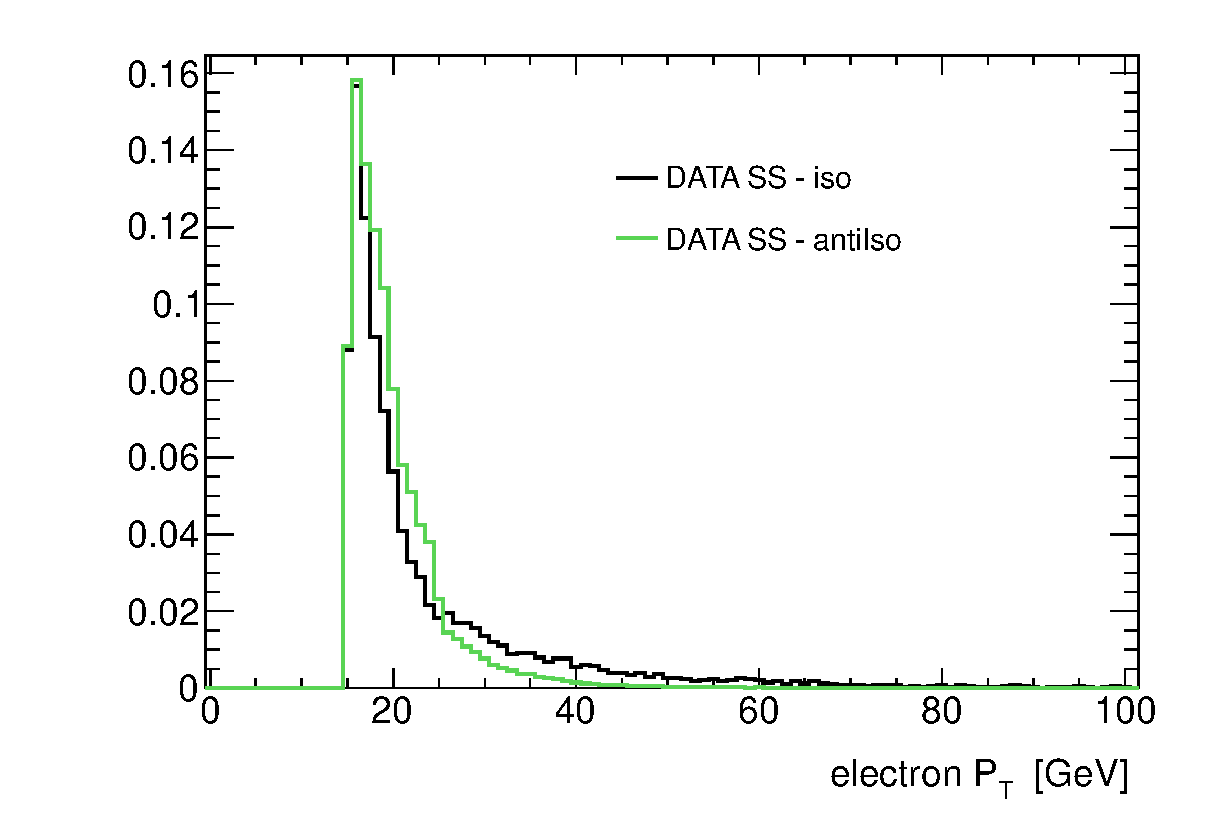
\includegraphics[width=9cm]{figure/ABCD_regionB_Vs_regionD}
	\end{center}
	\caption{Comparison of the electron \pt~distribution in region B and region D, showing the bias due to the trigger. 
	The histograms are normalised to the same area.}
	\label{fig:BvsD}
\end{figure}
%%%%	this table is not that useful

%\begin{table} [p]
%	\caption{Contribution to the different control regions from non-QCD background, after the preselection. }
%	\centering
%	\begin{tabular}{ c c c c c c c}
%%%%%%%%%%%%%%%%%%%%%%%%%%%%%%%%%%%%%%%%%%%%%%%%%%%%%%%%
%\hline
%Region  &  \Ztautau	 & $t\bar{t}$	 & W + jets	 & $Z \rightarrow ll$ + jets & Single Top 	& Dibosons \\ [0.5ex]
%\hline
%  B 	& 341 	$\pm$ 6	&	700$\pm$ 11	&	3398$\pm$ 180	& 830 $\pm$ 58	     &	178$\pm$ 8 		&   612$\pm$ 10  \\
%  C 	& 16 	$\pm$ 2	&	719$\pm$ 12	&	409$\pm$ 50	& 17 $\pm$ 4	     &	103$\pm$ 6		& 13$\pm$ 1 \\
%  D 	& 8	$\pm$ 2	&	539$\pm$ 10	&	49$\pm$	12	& 24$\pm$  7	     &	67$\pm$	 4		& 6$\pm$ 1 \\[1ex]
%\hline
%%%%%%%%%%%%%%%%%%%%%%%%%%%%%%%%%%%%%%%%%%%%%%%%%%%%%%%
%	\end{tabular}
%	\label{table:qcd_mc}
%\end{table}


%%%%%%%%%%%%%%%%%%%%%%%%%%%%%%%%%%%%%%%%%% PUT FINAL NUMBERS!!!!!!!!!!!!!!!! %%%%%%%%%%%%%%%%%%
\begin{table} [p]
	\begin{tabular}[c]{l r c c c c}
%%%%%%%%%%%%%%%%%%%%%%%%%%%%%%%%%%%%%%%%%%%%%%%%%%%%%%
\hline 
\hline 
Selection  &  		& B & C  & D &  \rqcd \\
\hline
Preselection 	&   Data	&6189			&604628			&312901		    &	1.929 $\pm$  	0.004		\\
	        &   non-QCD	&2510 $\pm$  180  	&1090 $\pm$   30  	&730	$\pm$ 35    &				\\
\hline
B-tag	     	&   Data	&419		&44619 			&27257		    &	1.64	$\pm$	0.01	\\
	     	&   non-QCD	&215 $\pm$  10	&310 $\pm$	12	&277 	$\pm$ 13    &				\\
\hline
$\Delta\phi(e-\mu)$  &   Data		&230		&38810 			&23316		    &	1.67	$\pm$	0.01	\\
	     &   non-QCD	&104 $\pm$ 6	&200 $\pm$	10	&175	$\pm$ 7	    &				\\
\hline
$\sum\cos\Delta\phi$ &   Data & 149		&31379 			&18779		    &	1.67	$\pm$	0.02	\\
	     &   non-QCD      & 67 $\pm$ 5	&127 $\pm$	8	&114 $\pm$	6   &				\\
\hline
$\sum H_T$ &   Data	      & 83		& 27781 		&15626		    &	1.78	$\pm$	0.02	\\
	&   non-QCD	      & 23 $\pm$  4	& 25 $\pm$	3	& 22 $\pm$   3	    &				\\ 
\hline
\SumLtMET &   Data	&71		&27735 	&15590		    &	1.78	$\pm$	0.02	\\
	     &   non-QCD	 & 10 $\pm$	3	& 22  $\pm$ 3		&18	$\pm$ 2	    &			\\
\hline
$\mmc > 0.$    &  Data	& 70	& 27634 	& 15522		    			    &	1.78	$\pm$	0.02	\\
	     &   non-QCD	& 9 $\pm$ 3	& 20  $\pm$ 3		&17	$\pm$ 2	    &			\\[1ex]
\hline
\hline
%%%%%%%%%%%%%%%%%%%%%%%%%%%%%%%%%%%%%%%%%%%%%%%%%%%%%%
	\end{tabular}
	  \caption{QCD background estimation as a function of the analysis selections for the b-tagged category. The yields for the different control regions, as well as the scaling factor \rqcd, are reported. The error on the \rqcd is statistical only.}
	\centering
	\label{table:qcd_yield_btag}
\end{table}


\begin{table} [p]
	\begin{tabular}[c]{l r c c c c}
%%%%%%%%%%%%%%%%%%%%%%%%%%%%%%%%%%%%%%%%%%%%%%%%%%%%%%%
\hline
\hline 
Selection  &  		& B & C & D &  \rqcd \\ 
\hline
Preselection 	&   Data	&6189			&604628			&312901		    &	1.929 $\pm$  	0.004		\\
	        &   non-QCD	&2510 $\pm$  180  	&1090 $\pm$   30  	&730	$\pm$ 35    &				\\
\hline
B-veto	     	&   Data	&5673		  & 558217 		& 284847		    &	1.960	$\pm$	0.004	\\
	     	&   non-QCD	&2220	$\pm$ 180 & 710 $\pm$ 30	& 415 $\pm$	30	    &				\\
\hline
$\Delta\phi(e-\mu)i$  &   Data		&4610		&532583 		&271404		    	    &	1.962	$\pm$	0.005	\\
	     &   non-QCD	&1700 $\pm$170	&580 $\pm$	30	& 345 $\pm$	30	    &				\\
\hline
$\sum\cos\Delta\phi$ &   Data& 3417	&486747 		& 247712	   		    &	1.965	$\pm$	0.005 	\\
	     &   non-QCD     & 1120  $\pm$ 100	& 370 $\pm$ 	20		& 230 $\pm$	20  &				\\
\hline
$\mmc > 0.$    &  Data		& 3177		& 479967 		& 244276	    	    &	1.965	$\pm$	0.005	\\
	     &   non-QCD	& 1000 $\pm$ 100	& 300  $\pm$ 17		&190	$\pm$ 20    &			\\[1ex]
\hline
\hline
%%%%%%%%%%%%%%%%%%%%%%%%%%%%%%%%%%%%%%%%%%%%%%%%%%%%%%%
	\end{tabular}
	\caption{QCD background estimation as a function of the analysis selections for b-veto category. The yields for the different control regions, as well as the scaling factor \rqcd, are reported. The error on the \rqcd is statistical only.}
	\centering
	\label{table:qcd_yield_bveto}
\end{table}



\begin{figure}[tp]
	\begin{center}
	     
	\subfigure[]{
		\includegraphics[page=1,width=0.49\textwidth]{figure/QCD/qcd_CR_emb.pdf}
	        }
	\subfigure[]{
  	\includegraphics[page=5, width=0.49\textwidth]{figure/QCD/qcd_CR_emb.pdf}
	}
	
	\end{center}
	\caption{\mmc distribution for QCD cross check regions defined in section \ref{sec:qcd} (a) and for the same CR when in addition one b-tagged jet is required (b). }
	\label{fig:ABCD_cr}
\end{figure}


Systematic uncertainties are assigned on the scaling factor \rqcd and on the shape of
the discriminating variable \mmc to take into account any correlation between isolation and charge 
of the leptons, details on the systematic uncertainty evaluation are addressed in Section~\ref{sec:Systematics}.





\subsection{$Z \rightarrow \tau\tau$ + Jets Background: Embedding Technique}
The background from \Ztautau decays is the major background to this analysis, a good uderstanding 
of it is then extremely important.
 Unfortunately, for a light Higgs boson, it is impossible to completely separate \Ztautau decays 
from the signal and signal free data control region cannot be defined.
However, thanks to the small Higgs coupling to muons, \Zmumu decays provide a good starting point to 
model \Ztautau events in a data-driven way. An hybrid Data-MC sample, known as "Embedding" is used to model the \Ztautau background: 
$\Zmumu$ candidates are selected in data, then the two muons from the $Z$ decay are substituted with the decay 
products from simulated taus, this means that also the energy in a cone around the muon is subtracted
and substituted with the one from tau decay, those taus have the same kinematics as the original muons. 
Further details may be found in \cite{Embedding, SMold}.

%The selection of the \Zmumu input data requires exactly two combined, opposite charged
%muons, where the leading muon has a transverse momentum $\pt > 20 \GeV$ and 
%the subleading muon $\pt > 15\GeV$. Both muons are requited to lie within $|\eta|<2.5$ and to be isolated with 
%$\ptcone 20/\pt<0.2$ (see Section~\ref{sec:presel}). Additionally 
%the invariant mass of the two muons is required to be in the range $M_{\mu\mu} > 40$ GeV.
%Once the muon pair events are selected, all tracks and calorimeter cells associated to the muons are 
%removed from the \Zmumu data event. Finally, the calorimeter cell energy and tracks from the simulated tau decays
%are added to the data event and the event is re-reconstructed.

%A set of corrections are applied to correct for the muon trigger efficiency, the muon reconstruction efficiency and other additional effects
%related to the original \Zmumu events. Finally, as the trigger is not emulated in the embedding sample, 
%an additional correction is applied to emulate the electron and muon trigger efficiencies in the final \Ztautau embedded events. 
%For a full description of the corrections and validation see \cite{SMnew}.

%The Embedding technique, which uses \Zmumu decays to 
%model \Ztautau events in a data-driven way, is described in Section~\ref{sec:data_mc}. 
There is no simulation of the trigger in the embedding samples, the event yield
is normalised to ALPGEN \Ztautau at preselection stage. Furthermore a set of corrections, as described in \cite{SMnew}, are
applied to unfold from the trigger and muon reconstruction efficiency of 
the original \Zmumu events, then trigger and reconstruction efficiency for muon and electron is emulated 
by the use of event weight.

The Embedding technique has been validated in several studies, detailed in~\cite{Embedding, SMnew}, which show a good description of 
data and \Ztautau MC by Embedding. In the context of this analysis, 
figures~\ref{fig:emb_vs_alp1} and \ref{fig:emb_vs_alp} show comparisons of various kinematic variables between
data, embedding and ALPGEN \Ztautau events at preselection. No significant deviation is seen 
between the \mmc distribution of the embedding and ALPGEN samples. 
However other relevant variables for this analysis, such as the \MET 
and the number of b-jets, are slightly better described by embedding. Additional plots are 
reported in appendix~\ref{appendix:additionalEmb}.

\begin{figure}[tp]
     \begin{center}

            \includegraphics[page=1, width=0.6\textwidth]{figure/bg_estimation/std_plots_emb.pdf}
\end{center}
    \caption{Comparison between the embedded \Ztautau and ALPGEN for $\mmc$ distributions.}
   \label{fig:emb_vs_alp1}
\end{figure}


\begin{figure}[tp]
     \begin{center}

           \includegraphics[page=2, width=0.6\textwidth]{figure/bg_estimation/std_plots_emb.pdf}
            \includegraphics[page=3, width=0.6\textwidth]{figure/bg_estimation/std_plots_emb.pdf}

    \end{center}
    \caption{Comparison between embedded \Ztautau and ALPGEN for $\MET$ and the number of b-tagged jets distributions.
	Data are superimposed, with the contribution of non-\Ztautau are subtracted.}
   \label{fig:emb_vs_alp}
\end{figure}


%plot comparing embedding and ALPGEN Et miss and b-tagging, data -MC not Ztautau and compare data alp and emb.

The Embedding sample is based on selecting \Zmumu candidates in data, the selections assure a rather 
pure \Zmumu sample, however further selections used in this analysis, for example the b-tagging requirements, 
could enhance the contamination fraction from other processes in the embedding sample. Hence dedicated studies have been
made to estimate the $t\bar{t}$ and QCD multi-jet contamination in the embedding sample.
The \ttbar~ contamination is estimated by evaluating the embedding sample yield in a two b-tag control region,
as described in Section~\ref{sec:top_est}. These events are assumed to be solely from $t\bar{t}$
and their yield in the signal region is extrapolated using POWHEG-PYTHIA $t\bar{t}$ simulation sample.
Table~\ref{table:emb_cont_tt} shows a summary for the top contamination in embedding and this contamination is hence taken to be negligible. The multi-jet contamination can be estimated starting 
from the embedding yield of opposite sign anti-isolated events (region C).
%one should not use SS regions because embedding already requires leptons to be OS, then would be biased
Assuming all events in this CR as QCD multi-jet events, the contamination in the SR 
can be estimated using the ABCD method (see Section\ref{sec:qcd}). The \rqcd factor 
used in this case is evaluated using a mu-mu final state CR with the same kinematics selections
used in the definition of the embedding sample. Table~\ref{table:emb_cont_qcd}
shows the estimated contamination of QCD multi-jet in embedding. 
We  consider contamination effects negligible.


\begin{table} [tp]
\centering
\begin{tabular}{c c c c c}
\hline
\hline
 & Embedding	& Transfer	& Estimated	& Contamination \\
 & yield in CR	& factor	& events in SR	&	\\		 [0.5ex]
\hline
b-tag & $84 \pm 9$  & $(2.6 \pm 0.1) \times 10^{-2}$ &  $2.2 \pm 0.2$&  0.5 \% \\
b-veto & $84 \pm 9$ & $(1.74 \pm 0.02) \times 10^{-1}$ & $15 \pm 2$ & 0.03 \% \\[1ex]
\hline
\end{tabular}
\caption{Evaluating embedding $t\bar{t}$ contamination using a two b-tag CR. The transfer factor is the
multiplicative factor that allows to estimate events in SR from the CR. }
\label{table:emb_cont_tt}
\end{table}

\begin{table} [tp]
\centering
\begin{tabular}{c c c c c}
\hline
\hline
 & Embedding	& Transfer	& Estimated	& Contamination \\
 & yield in CR	& factor	& events in SR	&	\\		 [0.5ex]
\hline
B-tag  & $12 \pm 3$ & $ (7 \pm 1) \times 10^{-3}$ &  $(8.4 \pm 0.3) \times 10^{-2}$ &  0.03 \% \\
B-veto & $390 \pm 20$ & $(2.5 \pm 0.1) \times 10^{-2}$ & $10.0 \pm 0.5$ & 0.02 \% \\[1ex]
\hline
\end{tabular}
\caption{Evaluating embedding contamination due to QCD multi-jet using ABCD method, 
the CR here is with OS anti-isolated events (region C). The transfer factor is the
multiplicative factor that allows to estimate events in SR from the CR, in this case is $N_{B} / N_{D}$
and is evaluated using mu-mu final state with the same kinematic selection used in the 
definition of the embedding sample. }
\label{table:emb_cont_qcd}
\end{table}




\section{Systematic Uncertainties}
\label{sec:Systematics}

This section describes the range of systematic uncertainties
that are relevant for this analysis. To account for differences in the detector responses between simulation and data a 
set of corrections are applied either at object reconstruction level and at event level. 
The uncertainties on such corrections are considered as detector-related systematic 
uncertainties and are detailed in section~\ref{sec:sys:sys_det}. 
Further systematic uncertainties related to data-driven methods for backgrounds estimation
are described in section~\ref{sec:sys_bg}.  For
samples which rely on MC simulation, theory-related
systematics, which include uncertainties on the cross-section and
uncertainties on the acceptance of analysis selections,  
are finally described in section~\ref{sec:sys_theory}.

Each single systematic can contribute separately to the uncertainty on the
final event yield and on the shape of the $\mmc$
distribution that is used as the discriminating variable for the limit derivation. These shape systematics are
documented in appendix~\ref{appendix:shapeNPs}. Systematic uncertainties that do not effect the
mass shape distribution and have an impact on the event yield of a samples of less than 0.5\% are 
neglected in the final limit calculations.
%hey infact do not have any significant effect on the final expected limits.


\subsection{Detector-related Systematics Uncertainties}
\label{sec:sys:sys_det}
Here systematic uncertainty related to object reconstruction and event 
corrections are addressed, those corrections are based on the measure of some relevant parameter, 
each of those parameters correspond to a "nuissance paremeter" in our probability model 
as described in Section~\ref{sec:ExclusionLimits}.
Each parameter is variated independently (one sigma up or down) according with its 
uncertainty and the impact on the analysis yield for each sample is evaluated.
In the following, detector related uncertainty are  described with some more details,
table~\ref{tab:ExpSys:btag} and~\ref{tab:ExpSys:bveto} briefly summarize the impact on the samples 
yield for the most significant systematic uncertainty considered. 


\paragraph{Luminosity}
The integrated luminosity of the 8 TeV data recorded at ATLAS during 2012 is measured to be $20.3 ~ fb^{-1}$ \cite{luminosity}, its uncertainty  is  2.8\%.

\paragraph{Pileup}
Simulated events are re-weighted to reproduce the average interactions per bunch crossing, $<\mu>$, seen in data. 
Those event weights has an uncertainty wich is propagated to each simulated sample.
%It has been seen
%that a proper description of the minimum bias vertex multiplicity is obtained if the $<\mu>$ 
%value in MC is first scaled by a factor of $1.11 \pm 0.03$ before re-weighting to match data. The uncertainty
%on this value is taken as a systematic uncertainty for the analysis.

\paragraph{Trigger Efficiency}
Trigger efficiency is corrected in simulation to match (as a mean value) the one in data, those correction weights 
are evaluated as a function of $\pt$ and $\eta$ of the leptons and have assciated uncertainties. 
Systematic uncertainties on both the single electron and electron-muon trigger efficiency are considered independently,  
those uncertainty range aproximately 1-2\%.

In the embedding sample, the trigger is emulated by applying weights to the event
topology in order to recover the right trigger efficiency, those weights are related to the one just described
and have similar uncertainty. Trigger efficiency uncertainty for Embedding are considered uncorrelated with 
the one of other samples.

\paragraph{Electrons}
Two types of uncertainty on reconstructed electron objects are considered:
the first are related to electron identification and reconstruction efficiencies ("Electron ID"), 
the second type are related to electron energy scale and resolution corrections.
The energy scale uncertainties are split into a set of six different nuisance parameters, 
however only few of them give a non negligible contribution, in particular two of them are found
to affect the shape of the \mmc distribution and are considered independently, those are the uncertainty
that arise from the $Z \rightarrow ee$ momentum measurement ("Electron Zee") 
and the one related to low momentum electrons ("Electron LOWPT"). 
We sum in quadrature all the other uncertainties related to energy scale and 
resolution ("Electron E.").

\paragraph{Muons}
The uncertainty on muon identification efficiency depends on the charge and momentum of the muon.
Typically these uncertainties are of the order of a fraction of percent, and are referred as "Muon ID". 
The uncertainties on the muon energy scale and resolution are considerd independently for the inner detector 
and muon spectrometer measurements, then are added in quadrature to eastimate the final effect ("Muon E").

\paragraph{Taus}
Hadronic tau object are only used in the analysis as a veto. Uncertainties on both tau energy scale 
and identification efficiency have been investigated and are found to be negligible for this analysis.

\paragraph{Jets}
The systematic uncertainties on the Jet Energy Scale (JES) are split up into multiple sets of nuisance parameters, which
are related to different effects and components, for example: the sensitivity to pileup or
to the flavour composition of the jet. The overall uncertainty on the JES ranges 
between 3\% and 7\%, depending on the $\pt$ and $\eta$ of the jet. To give an idea of the effect that these
uncertainty have on the analisis yield their sum in quadrature is reported in table~\ref{} ("JES"), 
this is just a simplification used here as illustration and in the limits extraction they are considered separately.
Systematic uncertainty due to jet resolution ("Jet Resolution") are obtained by smearing the jet energy 
according to its uncertainty.
%The recommendation \cite{TWIKI_JETMET} to propagate each individual 
% source of uncertainty through the full analysis is followed. In this analysis the reduced set of fourteen uncertainties, know as 
% \verb=InsituJES2012_14NP=, have been considered: these include two uncertainties for eta intercalibration, four pile-up 
% uncertainties, a high-$\pt$ uncertainty and an uncertainty for MC non-closure. Of these, only the terms "JES Effective 1", 
% "JES Effective 2" and "JES Effective 3", the pileup uncertainty as a function of the number of primary vertices ("JES Pileup-NPV") and the uncertainty due to the jet area ("JES Pileup-Rho") have a significant effect on the event yields. Additionally, 
% the uncertainty related to the fraction of quark to gluon jets ("JES Flav. Comp") and on the different response to them ("JES Flav. Resp.") are considered. The additional uncertainty assigned to the b-jet energy scale, referred as "JES B", is also 
% significant to this analysis. Uncertainties related to theory and modelling ("JES EtaModelling") also contribute to this 
% analysis. Finally the effect of the jet energy resolution ("JES Resolution") is evaluated applying a smearing to the jets, the 
% resulting effect on the yield is symmetrised.

\paragraph{b-Tagging} is described in chapter~\ref{chap:detector}. Corrections are applied to simulation
to match b-tagging efficiency with the one in data, uncertainties on the knowledge 
of the b-tagging efficiencies for the 70\% working point of the MV1 b-tagger are
considered in this analysis. 
Uncertainties for b-quark, c-quark and light or gluon initiated jets, are considered separately and referred respectively 
to as "B  Eff.", "C Eff." and "L Eff.". The tagging and mistagging efficiencies are considered to be totally anti-correlated. 

\paragraph{Missing Transverse Energy}
The effect of the energy scale
uncertainties for all the physics objects is propagated to the \met calculation.
In addition uncertainty on the energy scale and resolution due to the remaining 
calorimeter energy deposit, the so called ``soft-terms'', are considered. All the
uncertainty on \met are independently propagated through the analysis and are
added in quadrature, this final term is referred as "MET" uncertainty.


%\paragraph{Summary} A summary of the effect of the experimental and theoretical systematic uncertainties on signal and background yields for the b-tag and b-veto channels are shown in Table~\ref{tab:ExpSys:btag} and Table~\ref{tab:ExpSys:bveto}, respectively. It should 
%be noted that the gluon fusion  signal sample suffers of poor statistics in the b-tag category. 
%Hence, some of the yield differences reported are statistically dominated for these samples.
%%	As a solution the mean value between all the sample mass point can be taken as measure of the single systematic, 
%However the gluon fusion production mode has a negligible contribution in b-tag category.
	
\begin{table}[hp]
  \centering
  \begin{tabular}{lccccc}
    \hline\hline
      	      		   \multicolumn{6}{c}{ b-tag category uncertainties (\%)}  \\
     \hline
      Source             & Signal bbH & Signal ggH & \Ztautau &  Top 	& Other	 \\
    \hline
Electron SF  		 &2.3		   &2.0		     &	2.8    &	1.8	&2.0	 \\
Electron E.	  	 &0.7		   &1.2		     &0.5	     &0.5	&0.9	 \\
Electron LOWPT	  	 &0.4		   &0.0		     &0.4	     &0.1	&0.4	 \\ 
Electron Zee	  	 &0.3		   &0.6		     &0.4	     &0.6	&0.5	 \\
Muon ID 		 &0.3		   &	0.3	     &	0.3	     &	0.3	&0.3	 \\
Muon E.		  	 &0.5		   &7.7		     &0.1	     &0.1	&0.2	 \\
Trigger Single	Ele.  	 &0.7		   &0.5		     &0.5	     &0.8	&0.8	 \\
Trigger Dilepton  	 &1.0		   &1.2		     &1.4	     &0.6	&0.6	 \\
Embedding MFS	  	 &-		   &-		     &0.0	     &-		&-	 \\
Embedding Iso.	  	 &-		   &-		     &1.3	     &-		&-	 \\
JES Effective-1   	 &0.5		   &0.0		     &-		     &3.8	&2.3	 \\
JES Effective-2   	 &0.6		   &7.8 	     &-		     &5.5	&2.5	 \\
JES Effective-3   	 &0.5		   &0.0		     &-		     &2.2	&2.0	 \\
JES EtaModelling    	 &1.1		   &0.0		     &-		     &4.0	&2.1	 \\
JES Pileup-NPV	  	 &0.5		   &0.0		     &-		     &1.2	&0.3	 \\
JES Pileup-Rho	  	 &0.8		   &7.8 	     &-		     &2.8	&2.2	 \\
JES FlavComp.	  	 &1.2		   &6.3		     &-		     &2.1	&4.5	 \\
JES FlavResp.	  	 &1.3		   &0.0		     &-		     &1.4	&1.9	 \\
JES BJet	  	 &1.2		   &0.0		     &-		     &4.2	&1.2	 \\
JER		  	 &1.4		   &6.3		     &-		     &2.9	&3.0	 \\
B Eff		  	 &10.2		   &5.3		     &-		     &2.6	&5.0	 \\
C Eff		  	 &0.2		   &2.8		     &-		     &0.0	&1.2	 \\
L Eff		  	 &0.4		   &8.0		     &-		     &0.1	&1.2	 \\
Pileup			 &0.4		   &0.7		     &0.4	     &0.4	&0.9	 \\
MET 		  	 &0.7		   &11.0 	     &0.2	     &1.0	&1.2	 \\
Acceptance		 &		   &		     &		     &		&	  \\
Cross Section	  	 &-		   &-		     &5.0	     &5.5	&7.1	 \\
Luminosity	  	 &2.8 		   &2.8	 	     &2.8 	     &2.8 	&2.8 	 \\

    \hline
    \hline
  \end{tabular}
  \caption{Summary of the effect of the experimental and theoretical systematic uncertainties on the yields of the different
	%samples used  in the b-tag channel. Here "Other" refers to the sum of all the remaining samples: $\Wln$, 
	%diboson, $\Zll$ and single top. The signal samples listed here are b-associated production and gluon 
	fusion with $m_{A}=120$ GeV and $\tan\beta=20$. 
	 Systematic uncertainties with a negligible effect are are listed with a value of 0.0
	 and those that lead to a  shape uncertainty are noted with the symbol (\textbf{s}). 
	Note that the same naming convention is respected for the actual nuisance parameters in the limit framework.}

  \label{tab:ExpSys:btag}
\end{table}


\begin{table}
  \centering
  \begin{tabular}{lccccc}
    \hline\hline
      	      		   \multicolumn{6}{c}{ b-veto category uncertainties (\%)}  \\
     \hline
      Source             & Signal bbH & Signal ggH & \Ztautau &  Top 	& Other	 \\
    \hline
Electron SF  		 &2.4		   &2.3		     &2.9 (\bf{s})	     &1.4	&1.6	 \\
Electron E.	  	 &0.4		   &0.5		     &0.4	     &0.5	&0.9	 \\
Electron LOWPT	  	 &0.3		   &0.5		     &0.4 (\bf{s})	     &0.0	&1.2  \\ 
Electron Zee	  	 &0.4		   &0.4		     &0.4 (\bf{s})	     &0.1	&0.3	 \\
Muon ID 		 &0.3		   &0.3		     &0.3	     &0.3	&0.3	 \\
Muon E.		  	 &0.1		   &0.1		     &0.1	     &0.5	&0.5	 \\
Trigger Single	Lep.  	 &0.6		   &0.6		     &0.5	     &0.9	&0.9	 \\
Trigger Dilep.	  	 &1.0		   &1.0		     &1.3	     &0.2	&0.3	 \\
Embedding MFS	  	 &-		   &-		     &0.1 (\bf{s})	     &-		&-	 \\
Embedding Iso.	  	 &-		   &-		     &0.0 (\bf{s})	     &-		&-	 \\
JES Effective-1   	 &0.2		   &0.2		     &-		     &0.4	&0.4	 \\
JES Effective-2   	 &0.2		   &0.3		     &-		     &0.3	&0.5	 \\
JES Effective-3   	 &0.2		   &0.2		     &-		     &0.2	&0.3	 \\
JES EtaModelling    	 &0.1		   &0.1		     &-		     &0.1	&0.3	 \\
JES Pileup-NPV	  	 &0.3		   &0.1		     &-		     &0.1	&0.3	 \\
JES Pileup-Rho	  	 &0.3		   &0.2		     &-		     &0.5	&0.5	 \\
JES FlavComp.	  	 &0.1		   &0.2		     &-		     &0.2	&0.5	 \\
JES FlavResp.	  	 &0.2		   &0.4		     &-		     &0.3	&0.6	 \\
JES BJet	  	 &0.2		   &0.0		     &-		     &0.5	&0.1	 \\
JER		  	 &0.5		   &0.3		     &-		     &0.6	&0.3	 \\
B Eff		  	 &1.8		   &0.0		     &-		     &12.0	&0.8	 \\
C Eff	  		 &0.0		   &0.1		     &-		     &0.1	&0.0	 \\
L Eff	  		 &0.0		   &0.1		     &-		     &0.2 	&0.1	 \\
Pileup			 &0.5		   &0.8		     &0.4	     &0.3	&0.3	 \\
MET  		  	 &0.2		   &0.8 	     &0.1	     &0.2	&0.5	 \\
Acceptance		 &		   &		     &		     &		&	  \\
Cross Section	  	 &-		   &-		     &5.0	     &5.5	&5.9	 \\
Luminosity	  	 &2.8 		   &2.8	 	     &2.8 	     &2.8 	&2.8 	 \\

    \hline
    \hline
  \end{tabular}
  \caption{Summary of the effect of the experimental and theoretical systematic uncertainties on the yields of the different
	samples used  in the b-veto channel. Here "Other" refers to the sum of all the remaining samples: 
	$\Wlnu$, diboson, $\Zll$ and single top. The signal samples listed here are b-associated production 
	and gluon fusion with $m_{A}=120$ GeV and $\tan\beta=20$. 
	 Systematic uncertainties with a negligible effect are are listed with a value of 0.0
	 and those that lead to a  shape uncertainty are noted with the symbol (\textbf{s}). 
	Note that the same naming convention is respected for the actual nuisance parameters in the limit framework.}
 \label{tab:ExpSys:bveto}
\end{table}


%\subsection{Systematics for Data-Driven Background Estimation Methods} 
%\label{sec:sys_bg}

\subsection{\Ztautau Embedding Systematics}
An important element of the embedding method is the subtraction of the 
calorimeter cells associated with the muons in the original \Zmumu event and their substitution with those from the simulated tau
decays. To make a conservative estimate of the systematic uncertainty on this procedure, 
the energy of the subtracted cells is scaled up or down by 30\%. The analysis is repeated with those modified 
samples and the relative uncertainty is referred as EMB\_MFS. The effect of this uncertainty affects mainly the shape of the \mmc 
distribution, shown in figure~\ref{fig:EmbeddingShapeNPs}.

\begin{figure}[tp]
	\begin{center}
	\includegraphics[width=0.49\textwidth]{figure/systematics/emb_sys_BtagFull_MFS.png}
	\includegraphics[width=0.49\textwidth]{figure/systematics/emb_sys_NoBtagFull_MFS.png}
	\end{center}
	\caption{Embedding MFS systematic uncertainty impact on $\mmc$.}
	\label{fig:EMBMFS}
\end{figure}

%\begin{figure}[htp]
%     \begin{center}
%
%        \subfigure[]{%
%            \label{fig:mvis}
%            \includegraphics[width=0.45\textwidth]{figure/distributions/NP_Shape_EmbMFS_BVeto_mmc.pdf}
%	}
%	
%        \subfigure[]{%
%            \label{fig:mmc}
%            \includegraphics[width=0.45\textwidth]{figure/distributions/NP_Shape_EmbIso_BVeto_mmc.pdf}
%	}
%
%    \end{center}
%    \caption{Effect on the \mmc distribution of the embedding sample due to (a) the EMB\_MFS and (b) embedding isolation systematics. The plots are made after the full b-veto category selection.}
%   \label{fig:EmbeddingShapeNPs}
%\end{figure}

In the selection of the \Zmumu sample only a loose requirement on muon track isolation is required.
A different selection on the muon isolation may effect the selected sample by modifying the topology of the event, 
% since the requirement is indirectly acting also on the muon \PT, 
changing the non-\Zmumu contamination or the activity in the calorimeter. 
To estimate  the importance of these effects in our
embedding sample, the isolation selection on the muons in the original \Zmumu events is tightened,
%to $\ptcone 40/ \PT<0.06$ 
%and $\etcone 20/ \PT<0.04$, rather than the nominal selection of only $\ptcone 20/ \PT<0.2 $. 
a looser selection would have limited impact because of isolation requirements at trigger level.
The resulting uncertainty, referred to as EMB\_ISO, affects both the yield and the \mmc shape of 
the embedding samples, as shown in figure~\ref{fig:EmbeddingShapeNPs}. 

Finally, because the normalisation of the embedding sample is determined by the use of the ALPGEN sample, 
the relative cross section and luminosity uncertainties are assigned. In addition
all the detector-related systematic uncertainties relevant to the decay products of the simulated tau 
decay are propagated to the embedding sample.
 
\begin{figure}[tp]
	\begin{center}
	\includegraphics[width=0.49\textwidth]{figure/systematics/emb_sys_BtagFull_Iso.png}
	\includegraphics[width=0.49\textwidth]{figure/systematics/emb_sys_NoBtagFull_Iso.png}
	\end{center}
	\caption{Embedding Isolation systematic uncertainty impact $\mmc$.}
	\label{fig:EMBISO}
\end{figure}

\subsection{QCD Multi-Jet Systematics}

In this analysis the QCD multi-jet background is estimated via the ABCD method, as
described in Section~\ref{sec:qcd}. This technique relies strongly on
the assumption that the lepton isolation variables are independent from the
charge correlation between the two leptons. Systematic uncertainties
are assigned to take into account deviations from this assumption.
First we consider the correlation between \rqcd and the lepton isolation selections,
then we compare the result with an auxiliary method. 

Figure~\ref{fig:os_ss_ratio} shows the \rqcd factor, the ratio between the QCD 
yields in region C and D, as a function of the lepton isolation selections (red points).
%correlation is clearly visible. 
As described previously, the expectation from non-QCD backgrounds is subtracted from the data in regions C and D.
To estimate the uncertainty on the value of \rqcd  an additional transfer factor is defined as follows: $R_{QCD}^{iso}  = \hat{A} / \hat{B}$,
where  $\hat{A}$ and $\hat{B}$  are semi-isolated OS and SS regions defined with the lepton isolation larger than the standard requirement, 
but less than a sliding cut. Once more, the non-QCD contributions are subtracted from the data yields.
%$R_{QCD}^{iso}$ is an attempt to calculate a best estimate for the QCD transfer factor between isolated regions,
%which is in definitive the goal of the ABCD method. 
The regions $\hat{A}$ and $\hat{B}$ are chosen to be semi-isolated 
due to the high contamination of non-QCD background and possible signal in region A and B. 
Figure~\ref{fig:os_ss_ratio} shows $R_{QCD}^{iso}$ as a function of the lepton isolation selections (black points).
The difference between \rqcd and $R_{QCD}^{iso} $ in the vicinity of the standard cut value is then assigned as a systematic uncertainty on \rqcd. Using the point where the cuts on the lepton isolation are twice their standard values, a systematic uncertainty of 15\% is found.
The plot in Figure~\ref{fig:os_ss_ratio} is made at preselection level, similar plots using the full selection
for the two categories are in Appendix~\ref{appendix:qcd_additional}.

%for the definition of lepton isolations used in this analysis, the ratio is calculated in regions where the isolation requirements are reversed. Due to a high contamination of signal and non-QCD backgrounds, "semi-isolated" OS and SS regions are additionally defined, where the lepton isolation is larger than the standard requirement, but less than a sliding cut. These regions are labelled $\hat{A}$ and $\hat{B}$  for the semi-isolated OS and SS regions, respectively, and hence we can define $R_{QCD}^{iso}  = \hat{A} / \hat{B}$. The difference between \rqcd and $R_{QCD}^{iso} $ in the vicinity of our standard cut value is then assigned as a systematic uncertainty on \rqcd. Using the point where the cuts on the lepton isolation are twice their standard values, ie. the $x=100\%$ point on the graph, a systematic uncertainty of 15\% is found.

%An additional method considers calculating $\rqcd^{AB}$ as the ratio between the estimated QCD contributions in region A and B.
%These regions, however, suffers of large contribution of non-QCD background and possible signal contamination, 
%this method is then only used as a cross check. Table~\ref{table:MCsub} shows a comparison between \rqcd and  $\rqcd^{AB}$
%for the two category at an early stage of the cutflow where signal contamination is negligible, agreement is seen within statistical uncertainties.

An additional method, used as a crosscheck, considers calculating \rqcd as the ratio between the estimated QCD contributions in region A 
and B. Here the non-QCD contributions are once more subtracted from data. However the large contribution of this non-QCD background, 
along with lack of statistics and possible signal contamination, lead to this only being used as a cross check. Table~\ref{table:MCsub} shows 
a comparison between \rqcd and $\rqcd^{AB}$ for the two categories at the preselection stage of the cutflow, where signal contamination is negligible. 
Agreement is seen between \rqcd values in the two regions, within statistical uncertainties. 

%\footnote{This effect is maybe due to the use of a \PT dependent isolation variable that effects the quark-gluon fraction.}.
%Expectation for non-QCD backgrounds are subtracted as usual. 
%This effect however doesn't tell anything on the uncertainty of our
%measure of \rqcd, we want to measure instead what is the discrepancy (for each
%choosen isolation cut value) between \rqcd and the same factor calculated 
%flipping isolation requirements, i.e. using the isolated regions A and B, we call this factor $R_{QCD}^{iso}$. 
%Due to the high contamination of non-QCD backgrounds and signal in these regions we then define:
%OS and SS isolated regions $\hat{A}$ and $\hat{B}$ in wich the leptons isolation
%should be greather than the standard value but less of predefined quantity on the x axis 
%of the graph (black curve). In definitive we have $R_{QCD}^{iso}  = \hat{A} / \hat{B}$.
%We then assign as a systematics uncertainty the difference between the two curves (red and black) in the vicinity of our
%standard cut value (we use the point where the cut value is doubled, 100\% in the graph because 
%of statistical fluctuation), our estimate of the systematics uncertainty on \rqcd is then 15\%.
%The plot in Figure~\ref{fig:os_ss_ratio} is made at preselection level, similar plots using the full selection
%for the two categories are in Appendix~\ref{appendix:qcd_additional}.

%An additional method used as a crosscheck relies on the definition of "real-$\rqcd$" as the pure ratio between region A and B (non-QCD background
%estimate is subtracted from data in each regions), this would be the exact factor 
%that allows you to extrapolate yield from region B to SR, however it suffer of contamination by non-QCD backgrounds
%and lack of statistics.
%Table~\ref{table:MCsub} shows comparison between \rqcd and real-\rqcd
%for the two category at an early stage of the cutflow where signal contamination is negligible.
%Discrepancies are within statistical uncertainty and underline that an assignment of a  15\%
%uncertainty to the \rqcd factor is conservative.

 %How this is actually implemented in limits machinery
The actual implementation in the limit framework of the ABCD method follows that suggested in~\cite{ABCD}.
Here three free parameters are fitted: number of multi-jet events in region B, $N_{B}^{QCD}$, factor that extrapolates from SS region to OS regions, \rqcd, and the factor that 
extrapolates from isolated to anti-isolated regions $R_{BD}$. Neglecting signal contributions, the following 
equations can be written for the event yield of the B,C and D control regions:
%$$N_{B} = N_{B}^{BKG} + N_{B}^{QCD} $$ 
%$$N_{C} = N_{C}^{BKG} +  N_{B}^{QCD} \times \rqcd \times R_{BD} $$
%$$N_{D} =  N_{D}^{BKG} + N_{B}^{QCD} \times  R_{BD} $$
\begin{itemize}
\item[] $N_{B} = N_{B}^{BKG} + N_{B}^{QCD}$
\item[] $N_{C} = N_{C}^{BKG} +  N_{B}^{QCD} \times \rqcd \times R_{BD} $
\item[] $N_{D} =  N_{D}^{BKG} + N_{B}^{QCD} \times  R_{BD} $
\end{itemize}
where $N^{BKG}$ represent the prediction of  non-QCD background in the relative regions.
The estimate of multi-jet event yield in SR will be then $ N_{B}^{QCD} \times \rqcd $. This method is 
particularly powerful because in the best fit of \rqcd the statistical 
and systematics uncertainty for non-QCD backgrounds and data will be considered.


\begin{table} [tp]
	\begin{center}
	\begin{tabular}{l  c c c }
%%%%%%%%%%%%%%%%%%%%%%%%%%%%%%%%%%%%%%%%%%%%%%%%%%%%%%
\hline 
\hline
Selection  		&  \rqcd  			&  $\rqcd^{AB}$  		&  $R_{QCD}^{iso}$ \\ 
\hline
Preselection 		&   1.929 $\pm$     0.004	&	2.12 $\pm$ 0.17		&	2.22 $\pm$ 0.16	\\
B-veto			&  1.965   $\pm$   0.005    	& 2.10   $\pm$	0.16 		&	2.22 $\pm$ 0.16	\\
B-tag			&  1.78    $\pm$   0.02 	& 1.9   $\pm$	0.9 		&	2.0  $\pm$ 0.8	\\
\hline
\hline
%%%%%%%%%%%%%%%%%%%%%%%%%%%%%%%%%%%%%%%%%%%%%%%%%%%%%%
	\end{tabular}
	  \caption{Comparison between \rqcd, $\rqcd^{AB}$ and $R_{QCD}^{iso}$ for early stage in the cutflow, only b-tag and b-veto
	requirement are applied after preselections. Reported is statistical uncertainty only.}
	\label{table:MCsub}
	\end{center}
\end{table}


\begin{figure}[tp]
	\begin{center}
	\includegraphics[page=5,width=0.9\textwidth]{figure/QCD/qcd_plot.pdf}
	\end{center}
	\caption{OS/SS ratio as a function of lepton isolation variable selections. The selections are varied as a percentage relative to
	the standard lepton isolation cut values (0~in the plot). 
	%As an example the point at 100\% in the plot corresponds
	%to $\rqcd$ evaluated by increasing the isolation requirement by 100\% respect to the standard cut value.
	The red points show the anti-isolated scale factor $\rqcd$, i.e. the ratio between regions C and D.
	 The black points show the isolated SF, which is defined as the ratio between region $\hat{A}$ and $\hat{B}$, 
	 where the leptons have isolation values larger than the nominal value but smaller
	 than the sliding cut on X axis.
%	 taking the same example point at 100\%, than the double of the standard cut value.
	 }
	\label{fig:os_ss_ratio}
\end{figure}

The difference in \mmc shape observed between the OS and SS anti-isolated regions (C and D) is shown in Figure~\ref{fig:qcd_shape_unc}.
This effect is within the  uncertainty on \rqcd of the ABCD method, hence no correction factor is applied to the mass shape. We assume, however, that there could be the same 
shape difference in the isolated regions. Hence a shape uncertainty is assigned in the limit machinery to region B with this deviation. Further 
shape uncertainties due to non-QCD background subtraction are found to be negligible. The uncertainty due to the use of an isolation 
requirement at trigger level is discussed in Appendix~\ref{appendix:qcd} and is found to be negligible.


\begin{figure}[tp]
	\begin{center}
	\includegraphics[width=0.65\textwidth]{figure/QCD/shape_tag.png}
	\includegraphics[width=0.65\textwidth]{figure/QCD/shape_veto.png}
	\end{center}
	\caption{Shape differences for the b-tag and b-veto categories between the ABCD regions C and D.}
	\label{fig:qcd_shape_unc}
\end{figure}






\begin{table} [t]
\centering
\begin{tabular}{c c c }
\hline
\hline
Generator & Process & Uncertainty \\ [0.5ex]
\hline
ALPGEN & $Z \rightarrow \tau\tau / ee /\mu\mu$ & $\pm 5\%$ \\
POWHEG & \ttbar					& $\pm 5.5\%$\\
ALPGEN & $W  \rightarrow \tau\nu / e\nu /\mu\nu$&  $\pm  5\%$ \\
AcerMC & single top & $\pm 13 \%$ \\
HERWIG & dibosons & $\pm 6 \%$ \\
SHERPA & $bbA$/$h$/$H$  ($m_{A} \ge 120$~GeV)     & $-(<20)$\%,  $+(<9)$ \%\\
SHERPA & $bbA$/$h$/$H$  ($m_{A} =   110$~GeV)     & $-(<25)$\%,  $+(<9)$ \%\\
SHERPA & $bbA$/$h$/$H$  ($m_{A} =   100$~GeV)     & $-(<28)$\%,  $+(<9)$ \%\\
SHERPA & $bbA$/$h$/$H$  ($m_{A} =    90$~GeV)     & $-(<30)$\%,  $+(<9)$ \%\\
POWHEG & $ggA$/$h$/$H$  ($m_{A} \le 300$~GeV)     & $<$ 15\%\\  [0.5ex]
\hline \hline 
\end{tabular}
\caption{Cross-section uncertainties for background and signal samples.The reported signal samples are all for $\tan\beta = 20$.}
\label{table:sys_xsec}
\end{table}


\subsection{Theoretical Uncertainties}
\label{sec:sys_theory}
%\subsection{Simulated Cross-Section Uncertainties}

Uncertainties on the cross-sections that have been used to normalise
simulation samples to data are reported in
Table~\ref{table:sys_xsec}. These
uncertainties include contributions due to parton distribution
functions (PDFs), the choice of the value of strong coupling constant,
and the renormalisation and factorisation scales.  Furthermore the
uncertainties on signal cross-section depends on $\tan\beta$, the
Higgs boson type ($A$/$h$/$H$) and mass.

The effect of systematic uncertainties due to various MC tuning
parameters, underlying event and
lepton kinematic description is considered.
Since the effect on the invariant mass distribution of the di-tau system from these systematic
uncertainties is negligible (as an example see
Figure~\ref{fig:theory_mass} ), only the variation in
acceptance is considered as systematic uncertainty.
The acceptance uncertainties for the ALPGEN Z MC, used for the normalisation of the embedded sample, 
are estimated at lepton preselection to be 4\% \cite{2010SMLLSupportNote}.
%\footnote{A bit old result, to be reviewed. Depends also on the
%embedding choice}
Since additional selections are applied directly to the embedded sample, 
no further acceptance uncertainties is considered. Acceptance systematics on
$t\bar{t}$ simulated events are still to be determined. %\textcolor{red}{still to be added}.
%evaluated
%\footnote{also here is not totally clear yet} 
%by the difference between MC@NLO and POWHEG in
%the data-driven background estimate. 
%For other, single and dibosons
%production as well as single top production a 2\% uncertainty is
%assumed.
The acceptance uncertainties on diboson and single top production are assumed to be 2\%.
%\footnote{preliminary, this is following LEP-Had note, we
%  should cite some previous result here.}.
Uncertainties on signal acceptance have been estimated
by producing samples with varied MC generator parameters and evaluating, at
truth-level, the effect of analysis selections on leptons, taus and
jets. This truth-level study is implemented within the Rivet framework
\cite{RIVET}, where additionally b-tagging is performed by identifying b-quarks and applying
a weighting according to the estimated ATLAS b-tagging
efficiencies \cite{BtaggingScaleFactors}. The variation of the acceptance
with respect to the nominal MC tune has  been considered as
a source of systematic uncertainty. For signal a total acceptance 
uncertainty varies from 4\% to 30\% depending on $\mA$, production process 
and on the analysis category.

%The acceptance uncertainties of the two signal production modes are
%evaluated separately because of the use of different generators for each. For
%b-quark associated production, generated with SHERPA,
%the CKKW matching parameter $Q_{cut}$ has been varied from its default
%of $\sqrt{20 ~ GeV/E_{CMS}}$ to values of $\sqrt{15 ~ GeV/E_{CMS}}$
%and $\sqrt{30 ~ GeV/E_{CMS}}$. The factorisation scale was varied up
%and down by a factor of two and the renormalisation scale by a factor of
%10\%. Uncertainties due to the PDFs were determined by taking the RMS
%of the acceptance of the 52 error sets of the CT10 PDF set.  These
%effects are summarised in Table~\ref{table:sys_bba}. For a total
%uncertainty, all effects are summed in quadrature giving a total
%uncertainties that varies from 4\% to 30\% depending on $\mA$ and on the
%analysis category.  For gluon fusion production, generated with POWHEG
%and Pythia 8, the initial and final state
%radiation uncertainties were varied up and down, and the
%renormalisation and factorisation scales were varied simultaneously
%(the renormalisation scale by 10\% and the factorisation scale by factor 2\%).
%PDFs uncertainties were handled in the same way as for the $b$-quark
%associated production.  These variations are summarised in Table
%\ref{table:sys_gga}.  The uncertainties shown in Tables
%\ref{table:sys_bba} and \ref{table:sys_gga} are based on samples with
%$m_{A} = 120 \text{ GeV}$.  Results for the mass points 90, 200
%and 300 GeV are shown in Appendix \ref{appendix:additional} of this note.
 

\begin{figure}[tdp]
\begin{center}
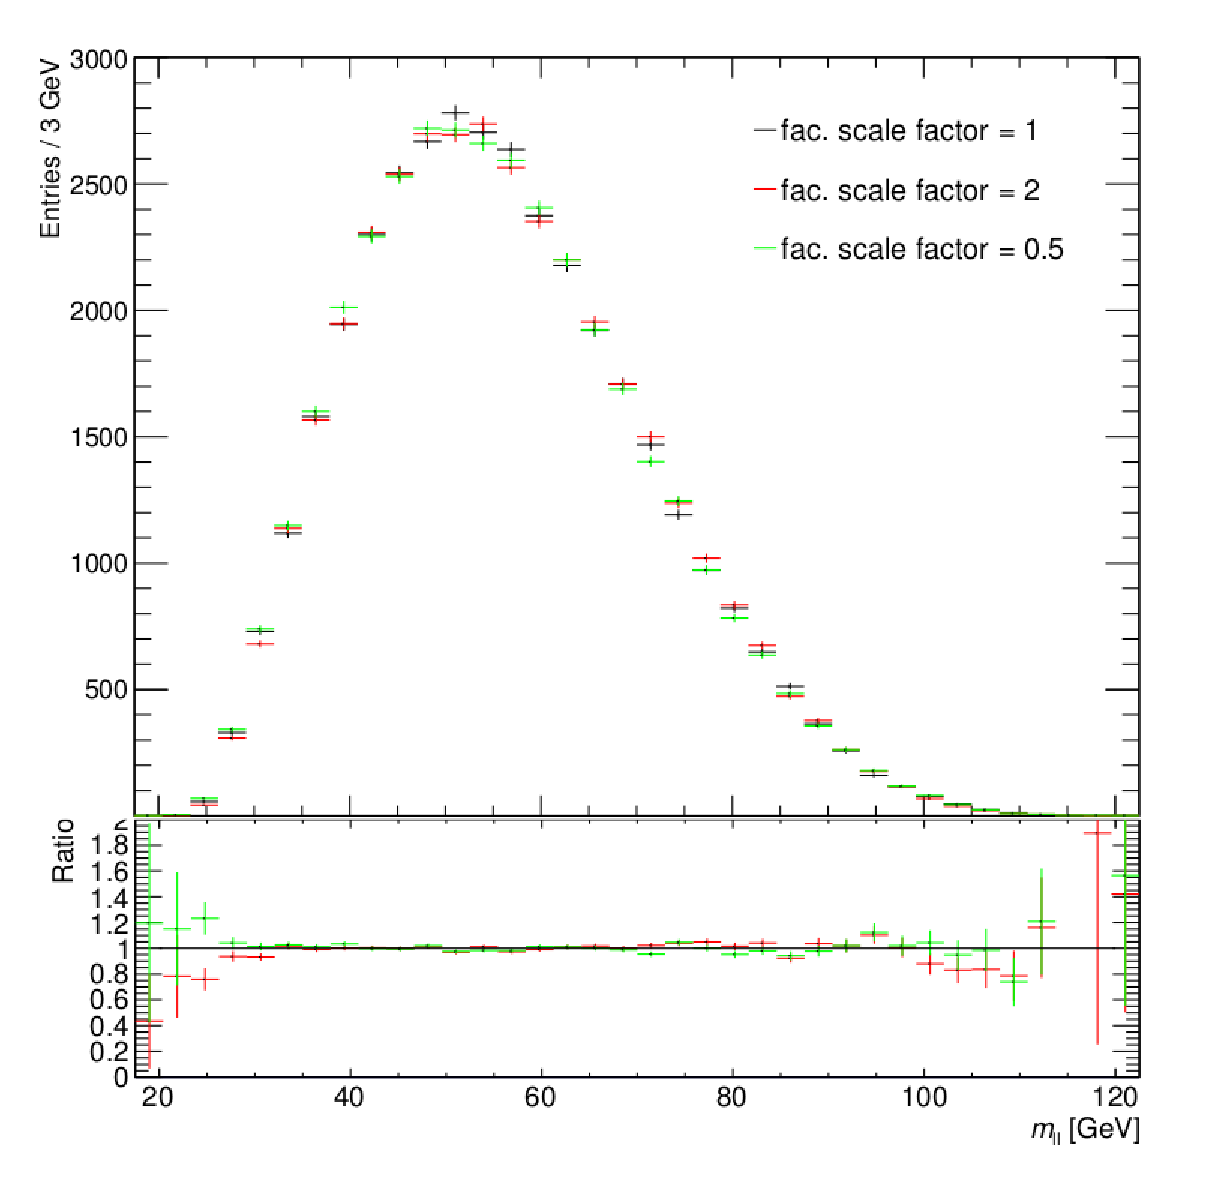
\includegraphics[width=8cm]{figure/facs_mll_bveto}
\end{center}
\caption{ Comparison of the visible mass of tau decay products after factorisation scale variation for the b-veto category on a gluon fusion signal sample.}
\label{fig:theory_mass}
\end{figure}


%\begin{table}[tdp]
%  \begin{center}
%   \label{table:sys_bba}
%   \begin{tabular}{lccccc}
%\hline \hline
% Event yields       & b-tag deviation [\%]  & b-veto deviation [\%] \\
%\hline
%CKKW down &    $ -3.1 \pm 0.9 $ &      $ 0.4 \pm 0.4 $ \\
%CKKW up &     $ -8.3 \pm 0.9 $ &      $ 2.9 \pm 0.4 $ \\
%Fac. scale down &    $ 15.5 \pm 1.0 $ &   $ -4.2 \pm 0.4 $ \\
%Fac. scale up &     $ -19.8 \pm 0.8 $ &    $ 5.6 \pm 0.4 $ \\
%Ren. scale down &      $ 0.4 \pm 0.9 $ &     $ -0.3 \pm 0.4 $ \\
%Ren. scale up &     $ 0.8 \pm 0.9 $ &      $ 0.5 \pm 0.4 $ \\
%PDF &     $\pm 0.1 $ 		& $\pm 0.2 $ \\
%\hline
%Total  (up) &     $ 13.5 \pm 1.6$ &                    $ 6.3 \pm 0.8$ \\
%Total  (down) &     $ -21.7 \pm 1.5$ &                    $ -4.2 \pm 0.6$ \\ 
%\hline \hline
%	\end{tabular}
%   \caption{Signal acceptances for several systematic deviations of the theory parameters contributing to the b-quark associated production of Higgs bosons. The different variations are added in quadrature to a total uncertainty on the signal acceptance in the b-tag and b-veto channels.}
%  \end{center}
%\end{table}
%
%
%\begin{table}[tdp]
%  \begin{center}
%   \label{table:sys_gga}
%    \begin{tabular}{lccccc}
 %   \hline \hline
% Event yields      &   b-tag deviation [\%] &   b-veto deviation [\%] \\
%\hline
%ISR up & $ 20.3 \pm 8.1 $ 		& $ -1.2 \pm 0.6 $ \\
%ISR down & $ 3.6 \pm 7.2 $ 		& $ 0.4 \pm 0.6 $ \\
%FSR up & $ 16.6 \pm 7.8 $ 		& $ -0.2 \pm 0.6 $ \\
%FSR down & $ -3.6 \pm 6.8 $	 	& $ -0.7 \pm 0.6 $ \\
%Ren./Fac. scales up & $ 9.4 \pm 7.5 $ 	& $ 0.0 \pm 0.6 $ \\
%Ren./Fac. scales down & $ 2.5 \pm 7.1 $ & $ -0.5 \pm 0.6$ \\
%PDF &     $\pm 0.0 $ &$\pm  0.1 $ \\
%\hline
%Total (up) &    $ 28.2 \pm 16.9 $ &     $ 0.4 \pm 0.6$ \\
%Total (down) &    $ -3.6 \pm 6.8 $ &     $ -1.5 \pm 1.2$ \\ 
%\hline \hline
%	\end{tabular}
%   \caption{Signal acceptances for several systematic deviations of the theory parameters contributing to the Higgs boson production through gluon fusion. The different variations are added in quadrature to a total uncertainty on the signal acceptance in the b-tag and b-veto channels.}
%  \end{center}
%\end{table}


\section{Results}

\subsection{LHC Procedure For Limits Setting}
\label{sec:limits}
Redefinition of marked poisson  with likelihood, comment on Histfactory

def of likelihood:
$$
\mathcal{L}(\text{data}|\mu, \boldsymbol{\theta}) = \text{Poisson(data} | \mu \cdot s(\boldsymbol{\theta}) + b(\boldsymbol{\theta})) 
	\cdot f(\boldsymbol{\theta} | \hat{\boldsymbol{\theta}})
$$

%and the $\text{Poisson(data} | \mu \cdot s(\boldsymbol{\theta})$ 
and the $\text{Poisson(data }| \mu \cdot s(\boldsymbol{\theta})) $
stands for a product of Poisson probabilities to observe  events in the bin \textit{i}
$$
\prod_{i} \frac{(\mu s_i +b_i)^{n_i}}{n_i!} ~ e^{-\mu s_i -b_i}
$$

To compiute the compatibility of the data with the $H_{0}$ and $H_{1}$ hypotesis, and then exclusion limits 
one needs to define a test statistic. The test statistic, which has already been defined in section~\ref{},
is a function of the data which returns a real value. One can in principle use any test statistic, however, 
given the size of the test (probability to reject the null hypotesis when is true) one would like to have 
a test statistic which has the highest power $1 - \beta$ possible (probability to reject the 
null hypotesys when it is false), this means that the test statistic should have 
different distribution for the two hypotesis under test. Figure~\ref{} shows an example
of the distribution of an hipotetical test statistic for two hypotesis.
It has been shown by Neuman-P~\cite{} that in case of simple hyptesis (probability model without any parameter),
then the test statistic with the highest power is the ratio of the likelihood calculated with the two hypotesis:
The standard procedure at the LHC is to use the following test statistic \cite{} based on the likelihood ratio:
$$
\tilde{q_{\mu}} ~ = ~ -2 \text{ln} ~ \frac{\mathcal{L}(\text{data}|\mu, \hat{\boldsymbol{\theta}}_{\mu})}{\mathcal{L}(\text{data}|\hat{\mu}, \hat{\boldsymbol{\theta}})}
\quad \text{with the constraint} \quad 0 \leq \hat{\mu} \leq \mu
$$
 where $\hat{\mu}$ and $\hat{\boldsymbol{\theta}}$ are the maximum likelihood estimators for $\mu$ and $\boldsymbol{\theta}$ given the data, 
whereas $\hat{\boldsymbol{\theta}}_{\mu}$ is the maximul likelihood estimator of $\boldsymbol{\theta}$ given the data but considering
a signal streght of value $\mu$. to be noted that $\tilde{q_{\mu}}$ is increasing with increasing disagreement between data and the $\mu$ hypotesis under test.
The procedure for limits setting follows five steps:
\begin{enumerate}
	\item The signal hypotesis with signal streght $\mu$ is assumed, under this assumpion a set of 
	\textit{pseudo-data} is generated for different values of $\mu$.

	\item  $\tilde{q_{\mu}}$ is calculated for each of the \textit{pseudo-dataset} and each signal hypotesis generating
	the expected probability density function for $\tilde{q_{\mu}}$ given $\mu$, 
	$\text{f}(\tilde{q_{\mu}} ~| ~ \mu, \hat{\boldsymbol{\theta}}_{\mu},H_1)$.

	\item One does the same thing foe the null hypotesis, generate pseudo-data with the distribution of background only and 
	generate  the $\text{f}(\tilde{q_{\mu}} ~ | ~ \mu = 0, \hat{\boldsymbol{\theta}}_{0}, H_0)$.

	\item Once one has the pdf for the signal and signal + background hypotesis one can define for a given dataset (that can be this time
	real data or again pseudodata)  two p-values, which are the probability to obtain data less compatible with the hypotesis in consideration:
	$$
	p_{s+b} = P(\tilde{q_{\mu}} > \tilde{q_{\mu}}^{observed} ~ | ~ H_1)  \quad \text{for any given value of} ~  \mu ~ \text{and}$$
	$$ 
	p_{b} = P(\tilde{q_{\mu=0}} > \tilde{q_{\mu=0}}^{observed} ~ | ~ H_0)
	$$
	Calculate the ratio of this two probability and get what is called the $CL_{s} = p_{s+b} / p_{b}$ \cite{}.

	\item If for a given $\mu$ is obtained $CL_{s} ~ \leq ~ \alpha $ one states that the signal hypotesis (with that $\mu$) 
	is excluded with (1 - $\alpha$) $CL_{s}$ confidence level. To get the 95\% confidence level upper limit on $\mu$,
	denoted as $\mu^{95}$ one adjust $\mu$ until $CL_{s} = 0.05$. 
\end{enumerate}
This is a quite complicated prescription, however it has simple explaination in terms of confidence intervals:

For each $\mu$ is possible to define $\tilde{q_{\mu}}^{95}$ for which the probability P$(\tilde{q_{\mu}} > \tilde{q_{\mu}}^{95} ~ | H_1$ ) = 5\%,
	this means that if $H_1$ is true, this hypotesis will be rejected in 5\% of the cases.

 For each pseudo-data sample one can calculate then $\mu^{95}$, which is the biggest value of $\mu$ which gives $\tilde{q_{\mu}} > \tilde{q_{\mu}}^{95}$

 Generate a large set of pseudo-data under the hypotesis $H_{0}$ and calculate  $\mu^{95}$ for each of them, by costruction one would have
	that if $H_1$ is true for $\mu > \mu^{95}$ one has $\tilde{q_{\mu}} > \tilde{q_{\mu}}^{95}$ only 5\% of the cases.
	
So one it is said that the $\mu > \mu^{95}$ are excluded by data under the hypotesis $H_1$ at 95\% of Confidence Level, meaning that 
for value of $\mu > \mu^{95}$  one would reject the $H_1$ when is true at most 5\% of the time. 

\subsection{Exclusion Limits}
The procedure described in section~\ref{sec:limits} is actually the one which was used for the SM Higgs, for the MSSM there is a further 
complication: the cross section and the masses of $h$ and $H$ depends on $m_A$ and $\tan \beta$, then one has to consider in the signal 
model three Higges for which in a particular scenario the masses and cross section are defined for a given point in the $\tan \beta - m_A$
plane, so the procedure described previously has to be repeated for each point in that plane. For a given scenario, 
a point in the  $\tan \beta - m_A$ plane is excluded with 95\% $CL_{s}$ confidence level if $\mu^{95} \leq 1$ for that point. 
Only a limited number of $\tan \beta - m_A$ points are gerated, a linear interpolation is used to determine the $\tan \beta$ excluded for a given
$m_A$.

Add some part of limits of the note.

 

\subsection{Summary}



%trackjets
%\chapter{Prospects for Neutral MSSM Higgs Search Improvement}

The neutral MSSM Higgs search, described in the previous chapter, 
suffers strongly of poor jet reconstruction efficiency and  b-tagging performance due to the particular phase space
required, this bound the potential of this search, improoving b-tagging
would result in a major improvement of the search sensitivity. 
This chapter investigates an alternative to the commonly used calorimeter jets in ATLAS, 
which is trackjets b-tagging. 
The prospects for successfully use trackjets b-tagging in the future neutral MSSM Higgs searches are reported,
b-tagging on trackjets was never attempted before.
Section\ref{bla} describes this and that...


\clearpage

\section{Introduction to Trackjets}
% reasonable intro + ++ 
This problematic has two sources:
- The ATLAS calorimeter is not a sampling calorimeter, this means that responses differently 
for Hadrons and for leptons, has different responses to electromagnetic and hadronic shower.
The Calorimeter cells are calibrated in energy using response to electromagnetic showers, to 
know the energy of the original parton that initiated the jet there are different procedure 
to calibrate the Jets offline which are called in short Jet Energy Scale (JES) corrections \cite{}, 
which make use of MC simulation.
Due to the high amount of pileup and ambient energy density in the events, jets are calibrated % also other problems: underlying event ecc..
from 20 GeV in $\pt$, this means that currently is not possible with calorimeter jets to access the
low transverse momentum phase space.

\begin{figure}[tp]
     \begin{center}

            \includegraphics[width=0.49\textwidth]{figure/trackjet/bbA_pt.png}
            \includegraphics[width=0.49\textwidth]{figure/trackjet/top_pt.png}

    \end{center}
    \caption{Cormparison of simulated b-hadron distribution for signal b-associated production events (left) and $\ttbar$ events (right).
	The red line in the figure shows the acceptance region due to calibrated jet $\pt$ requirements.}
   \label{fig:bjetDistro}
\end{figure}

The neutral MSSM Higgs search, as described in chapter~\ref{chap:anal}, splits the dataset in two category
by means of the presence or the absence of a b-tagged jet, the b-tagged category is optimized for the b-associated production 
mechanism, in which the Higgs is produced in association with two b-jets. Figure~\ref{fig:bjetDistro} shows a comparison 
between $\pt$ spectrum of simulated b-hadron in b-associated Higgs  and $\ttbar$ events, the signal prefers b-hadron with 
relatively low transverse momentum,  jet calibration invoqe jet $\pt > 20$ GeV removing a large fraction of possible
signal candidate, many of the b-associated production signal events falls in fact in the b-veto category, making 
the separation not so effective.
The low $\pt$ spectrum is actually quite challenging, jet reconstruction efficiency and calibration set then a lower limit
to the signal sensitivity in the b-tag category.
Another challenge to this search are the poor b-tagging performance at low transverse momentum, for the a fixed tagging point of the 
MV1 tagger the b-tagging efficiency drops, in fact,  rapidly  with jet $\pt$ reacing a minimum of 50\% at 20 GeV \cite{BtaggingScaleFactors,BtaggingScaleFactorsNew}
(using as tagging point the 70\% point).

A solution to the jet reconstruction efficiency is to use, instead of calorimetric jets (calo-jet), track-jet , which are as well
anti-kt object (see chapter\ref{chap:detector}) but constructed using inner detector tracks as building blocks, not calorimeter cells.
Jets in the ATLAS reconstruction software are reconstructed by clustering foru vector objects (calorimeter energy cluster, tracks, 
truth particle, etc.) in the $\eta - \phi$ plane. In the case of clustering tracks, however, it is possible to take advantege of
the longitudinal (\emph{z}) impact parameter information provided by the inner detector and build track-jets in three dimensions 
$\eta - \phi - z$. Track-jets will then contains only tracks originating from the same interaction point (reconstructed vertex).
Even thoug for calorimeter jet is possible to use the JVF, track-jets result to be more resistant to decrease in performance in the
presence of pile-up, thus particolarly important in b-tagging, which depends on the determination of the jet-axis. 
B-tagging has been never tested before on track-jets, in the following, the first study of b-tagging over track-jets performances is reported. 



%as shown if figure~\ref{





%\subsection{Motivation}
%\subsection{Definition of Trackjet}
\section{Trackjet Performance}
\subsection{B-tagging Performance}
\subsection{Comparison Calo-jet Track-jet}
\subsection{Impact of Trackjet to the Analysis} % A new Hope
\subsection{B-Discriminant} % variable to enhance low pT b-tagging

\section{Systematic Uncertainties on Trackjets}
\subsection{General discussion}
\subsection{Track Subtraction Method} %general description of the method
\subsection{Track Subtraction Validation} %confermo che l'effetto di Ex material e' solo efficiency
\subsection{Track Subtraction Results}





%\section{Acknowledgements}

%%%%%%%%%%%%%%%%%%%%%%%%%%%%%%%%%%%%%%%%%%%%%%%%%%%%%%%%%%%%%%%%%%%%%%%%%%%%%%%
% Bibliography
%%%%%%%%%%%%%%%%%%%%%%%%%%%%%%%%%%%%%%%%%%%%%%%%%%%%%%%%%%%%%%%%%%%%%%%%%%%%%%
%\clearpage
\bibliography{tesi}

%%%%%%%%%%%%%%%%%%%%%%%%%%%%%%%%%%%%%%%%%%%%%%%%%%%%%%%%%%%%%%%%%%%%%%%%%%%%%%%
% Technical Aspects
%%%%%%%%%%%%%%%%%%%%%%%%%%%%%%%%%%%%%%%%%%%%%%%%%%%%%%%%%%%%%%%%%%%%%%%%%%%%%%%

\newpage
\appendix
\chapter{Additional QCD Studies}\label{appendix:qcd}

\section{Trigger Bias}

The single electron trigger (\verb=EF_e24vhi_medium1=) used in this analysis includes the following isolation cut: $\ptcone20 / \PT < 0.1$.
This means that the kinematical distributions in the anti-isolated ABCD regions will biased due to a reduced efficiency for high \pt~ electrons. This unwanted feature may potentially effect the \rqcd factor, as the OS/SS ratio may differ due to different \PT~ spectrum. 
To check the effect on \rqcd the ABCD method has been repeated using the \verb=EF_e24vh_medium1= trigger, which doesn't include isolation and hence is prescaled in 2012 8 TeV data. The prescale of a factor around 100 has been taken in consideration using trigger information stored in D3PD. Figure \ref{fig:prescale} shows 
\ptcone distribution for the standard and test triggers. The comparable event yields in the region $\ptcone20 / \PT < 0.1$ show that the prescale normalisation for the test trigger has been correctly accounted for.

Figure \ref{fig:trigRatio} shows the behaviour of \rqcd factor as a function of isolation variable for the two triggers under test.
As the deviations are within statistical uncertainty,  we conclude that the isolation requirement used at trigger level does not influence
the OS/SS ratio. Hence no further systematic uncertainty is assigned.



\begin{figure}[t]
\begin{center}
\includegraphics[width=9cm]{figure/appendix/trigger_comp.png}
\end{center}
\caption{\ptcone / \PT distribution for the analysis standard trigger and  its corrispective without isolation requirement,
this second trigger is rescaled according to prescales information.} 
\label{fig:prescale}
\end{figure}

\begin{figure}[t]
\begin{center}
\includegraphics[width=0.49\textwidth]{figure/appendix/trig_comp_ptcone3.png}
\includegraphics[width=0.49\textwidth]{figure/appendix/trig_comp_etcone3.png}
\end{center}
\caption{\rqcd  as a function of (a) \ptcone / \PT and (b) \etcone /PT for the electron triggers with and without isolation requirement.} 
\label{fig:trigRatio}
\end{figure}

\clearpage

\section{QCD Additional Plots}
\label{appendix:qcd_additional}

\begin{figure}[h!]
\begin{center}
\subfigure[]{
\includegraphics[width=0.45\textwidth]{figure/QCD/qcd_plot_1.pdf}
}
\subfigure[]{
\includegraphics[width=0.45\textwidth]{figure/QCD/qcd_plot_2.pdf}
}
\subfigure[]{
\includegraphics[width=0.45\textwidth]{figure/QCD/qcd_plot_4.pdf}
}
\subfigure[]{
\includegraphics[width=0.45\textwidth]{figure/QCD/qcd_plot_3.pdf}
}
\end{center}
	\caption{OS/SS ratio as a function of lepton isolation variable selections after the requirement of (a) zero b-jets, (b) the full b-veto category selection, 
	(c) of a b-jet, (d) the full b-tag category selections. The isolation selections are varied as a percentage relative to
	the standard lepton isolation cut values (0~in the plot). 
	%As an example the point at 100\% in the plot corresponds
	%to $\rqcd$ evaluated by increasing the isolation requirement by 100\% respect to the standard cut value.
	The red points show the anti-isolated scale factor $\rqcd$, i.e. the ratio between regions C and D.
	 The black points show the isolated SF, which is defined as the ratio between region $\hat{A}$ and $\hat{B}$, 
	 where the leptons have isolation values larger than the nominal value but smaller
	 than the sliding cut.
%	 taking the same example point at 100\%, than the double of the standard cut value.
	 }
\end{figure}




\chapter{Additional Plots and Results}\label{appendix:result}

\begin{figure}[!h]
  \centering
  \includegraphics[width=0.7\textwidth]{figure/limits/comb_reg_spin.pdf}
  \caption{Expected and observed  exclusion limits at the $95\%$ $CL_s$ confidence-level for MSSM Higgs bosons production 
   interpreted in the  $m_A - \tan\beta$ parameter space of the $m_h^{max}$ scenario. 
	Combined result of the  b-tagged and b-vetoed category is shown.}
\end{figure}

\begin{figure}[tp]
  \centering
  \includegraphics[width=0.6\textwidth]{figure/limits/tag_final.pdf}
  \includegraphics[width=0.6\textwidth]{figure/limits/veto_reg_spin.pdf}
  \caption{Expected and observed  exclusion limits at the $95\%$ $CL_s$ confidence-level for MSSM Higgs bosons production 
   interpreted in the  $m_A - \tan\beta$ parameter space of the $m_h^{max}$ scenario in the   b-tagged (top) and b-vetoed (bottom) category.}
\label{fig:limit_extract_combined2}
\end{figure}

\begin{figure}[!hp]
     \begin{center}
	
    \subfigure[]{		
            \includegraphics[ width=0.6\textwidth]{figure/paper/limit_comb_2d_lightstau.pdf}
	}
    \subfigure[]{		
            \includegraphics[ width=0.6\textwidth]{figure/paper/limit_comb_2d_tauphobic.pdf}
	}
    \end{center}
    \caption{Expected (dashed line) and observed (solid line with markers) 95\% CL upper limits on $\tan\beta$ as a function of $m_A$. 
	The upper limits are shown in for the statistical combination of all channels in (top) the light stau and (bottom) the tauphobic
	MSSM benchmark scenarios (see Section~\ref{sec:benchmark}). 
	The vertical dashed line at 200 GeV indicates the transition point between low and high mass categories~\cite{yuppy}.} 

\end{figure}





\begin{figure}[!h]
     \begin{center}
	
            \includegraphics[page=3, width=0.47\textwidth]{figure/final_plots/Bveto_final.pdf}
            \includegraphics[page=4, width=0.47\textwidth]{figure/final_plots/Bveto_final.pdf}
            \includegraphics[page=6, width=0.47\textwidth]{figure/final_plots/Bveto_final.pdf}
            \includegraphics[page=9, width=0.47\textwidth]{figure/final_plots/Bveto_final.pdf}
    \end{center}
    \caption{ Observed and expected distribution for different kinematical variables after full selection of the b-tagged category.
	 In the ratio, the yellow and red band represents the systematic and statistical uncertainty in the background model prediction, 
	respectively,  while the error bars respresent the statistical uncertainty of data.}
\end{figure}

\begin{figure}[!p]
     \begin{center}
	
            \includegraphics[page=9, width=0.47\textwidth]{figure/final_plots/BTag_fulll.pdf}
            \includegraphics[page=1, width=0.47\textwidth]{figure/final_plots/BTag_fulll.pdf}
            \includegraphics[page=2, width=0.47\textwidth]{figure/final_plots/BTag_fulll.pdf}
            \includegraphics[page=6, width=0.47\textwidth]{figure/final_plots/BTag_fulll.pdf}
    \end{center}
    \caption{ Observed and expected distribution fori different kinematical variables after full selection of the b-tagged category.
	 In the ratio, the yellow and red band represents the systematic and statistical uncertainty in the background model prediction, 
	respectively,  while the error bars respresent the statistical uncertainty of data.}
\end{figure}


\clearpage

\chapter{Further Details on Limit}
\label{appendix:limit}

\section{The ABCD Method }
%How ABCD  is actually implemented in limits machinery
The actual implementation in the limit framework of the ABCD method follows that suggested in~\cite{ABCD}.
The control data samples B,C and D are considered as additional channels to be statistically combined
to two the signal event category. Three free parameters are fitted in B,C and D channels which are: the 
number of multi-jet events in the data sample B, $N_{B}^{QCD}$, the factor \rqcd 
and the factor that extrapolates from isolated to anti-isolated data control samples $R_{BD}$. Neglecting signal contributions, 
the following equations can be written for the event yield of the B,C and D control data samples:
%$$N_{B} = N_{B}^{BKG} + N_{B}^{QCD} $$ 
%$$N_{C} = N_{C}^{BKG} +  N_{B}^{QCD} \times \rqcd \times R_{BD} $$
%$$N_{D} =  N_{D}^{BKG} + N_{B}^{QCD} \times  R_{BD} $$
\begin{itemize}
\item[] $N_{B} = N_{B}^{BKG} + N_{B}^{QCD}$
\item[] $N_{C} = N_{C}^{BKG} +  N_{B}^{QCD} \times \rqcd \times R_{BD} $
\item[] $N_{D} =  N_{D}^{BKG} + N_{B}^{QCD} \times  R_{BD} $
\end{itemize}
where $N^{BKG}$ represent the prediction of  non-QCD background in the relative data samples.
The estimate of multi-jet event yield in the signal sample will be then $ N_{B}^{QCD} \times \rqcd $. This method is 
particularly powerful because in the best fit of \rqcd the statistical 
and systematics uncertainty for non-QCD backgrounds and data are considered.

\clearpage

\section{Shape Systematics} \label{appendix:shapeNPs}

\begin{figure}[!h]
     \begin{center}
	\subfigure[]{	
            \includegraphics[width=0.47\textwidth]{figure/distributions/NP_Shape_ElecSF_BVeto_mmc.pdf}
	}
	\subfigure[]{	
            \includegraphics[width=0.47\textwidth]{figure/distributions/NP_Shape_ElecLowPt_BVeto_mmc.pdf}
	}
	\subfigure[]{	
            \includegraphics[width=0.47\textwidth]{figure/distributions/NP_Shape_ElecZee_BVeto_mmc.pdf}
	}
    \end{center}
    \caption{Effect on the \mmc distribution of the embedding sample due to the (a) the electron reconstruction and identification systematics, (b) the electron low \pt~ energy scale systematic and (c) the electron Zee energy scale systematic. The plots are made after the full b-veto category selection. Plots 
	provided by Matthew Backingham.}
\end{figure}

\clearpage

\section{Additional Limit Checks}
During the limit derivation, the systematic uncertainties (translated in term of nuisance parameter) are fitted to the data,
several checks are have been performed to ensure the quality of our statistical model.
If some of the nuisance parameters are significantly different from their nominal value 
(ie before fit), it can be symptomatic of an important mis-modelling and must be carefully scrutinised.
Also the correlation between the nuisance parameter and the signal strength (which reflects the degeneracy of the fit) 
is an important element to keep under control, in fact it reflects how well the data can constraint the nuisance parameters.
Finally, to have a feeling of the behaviour of the likelihood at its minimum one can check 
the negative log likelihood profile in each nuisance parameter direction. 
We performed all this checks using the package NuisanceCheck-00-00-05 described in \cite{NPcheck}.

The signal and background model with the signal normalisation free (unconditional fit) is fitted to the data,
in the following example plots the signal is assumed for the mass point mA~=~120 GeV, tan$\beta$~=~20,  
The difference between the post fit and pre-fit value of the nuisance parameter along with their errors is shown in Figure~\ref{fig:np_pull_comb}
for the combination between the two categories.
Figure~\ref{fig:np_correlation_comb} shows the correlation matrix between the nuisance parameters for the combination between the two channels.
Figure~\ref{fig:llh_1}-\ref{fig:llh_3} shows the behaviour of the likelihood at its minimum for 
each of the nuisance parameters (while a nuisance parameter is investigated the other are kept constant) for the combination between the channels.
%%%%%%%%%%%%%%%%%%%%%%%%%%%%%%%%%%%%%%%%%%%%%%% PULLS %%%%%%%%%%%%%%%%%%%%%%%%%%%%%%%%%%%%%%%%%%%%%%%%%%%%%%%%%%

\begin{figure}[htp]
     \begin{center}

            \includegraphics[width=\textwidth]{figure/np_check/120_comb_pulls.pdf}
            %\includegraphics[width=\textwidth]{figure/np_check/pulls_combined.pdf}
    \end{center}
    \caption{ Pulls for nuisance parameter considered in the fit,  mA = 120 GeV, tan$\beta$ = 20, combination between the two channel. These pulls are obtained with
	NuissanceCheck package, using asymptotic approximation.} 
    \label{fig:np_pull_comb}
\end{figure}
%%%%%%%%%%%%%%%%%%%%%%%%%%%%%%%%%%%%%%%%%%%%%%%  %%%%%%%%%%%%%%%%%%%%%%%%%%%%%%%%%%%%%%%%%%%%%%%%%%%%%%%%%%

%%%%%%%%%%%%%%%%%%%%%%%%%%%%%%%%%%%%%%%%%%%%%%% CORRELATION MATRIX %%%%%%%%%%%%%%%%%%%%%%%%%%%%%%%%%%%%%%%%%%%%%%%%%%%%%%%%%%
\begin{figure}[htp]
     \begin{center}

           \includegraphics[width=1.1\textwidth]{figure/np_check/matrix_comb_120.pdf}
           %\includegraphics[width=1.1\textwidth]{figure/np_check/matrix_combined.pdf}
    \end{center}
    \caption{ Correlation matrix for nuisance parameters considered in the fit.  The point mA = 120 GeV and tan$\beta$ = 20 is 
	considered for the combination of the b-tag and b-veto channels. This correlation matrix is obtained with 
	NuissanceCheck package, using asymptotic approximation.} 
    \label{fig:np_correlation_comb}
\end{figure}
%%%%%%%%%%%%%%%%%%%%%%%%%%%%%%%%%%%%%%%%%%%%%%%  %%%%%%%%%%%%%%%%%%%%%%%%%%%%%%%%%%%%%%%%%%%%%%%%%%%%%%%%%%

%%%%%%%%%%%%%%%%%%%%%%%%%%%%%%%%%%%%%%%%%%%%%%% llh SCANS %%%%%%%%%%%%%%%%%%%%%%%%%%%%%%%%%%%%%%%%%%%%%%%%%%%%%%%%%%

\begin{figure}[htp]
     \begin{center}

            \includegraphics[page=8,width=0.3\textwidth]{figure/np_check/comb_LLHscan_f.pdf}
            \includegraphics[page=9,width=0.3\textwidth]{figure/np_check/comb_LLHscan_f.pdf}
            \includegraphics[page=10,width=0.3\textwidth]{figure/np_check/comb_LLHscan_f.pdf}\\
            \includegraphics[page=11,width=0.3\textwidth]{figure/np_check/comb_LLHscan_f.pdf}
            \includegraphics[page=12,width=0.3\textwidth]{figure/np_check/comb_LLHscan_f.pdf}
            \includegraphics[page=13,width=0.3\textwidth]{figure/np_check/comb_LLHscan_f.pdf}\\
            \includegraphics[page=14,width=0.3\textwidth]{figure/np_check/comb_LLHscan_f.pdf}
            \includegraphics[page=15,width=0.3\textwidth]{figure/np_check/comb_LLHscan_f.pdf}
            \includegraphics[page=16,width=0.3\textwidth]{figure/np_check/comb_LLHscan_f.pdf}\\
            \includegraphics[page=17,width=0.3\textwidth]{figure/np_check/comb_LLHscan_f.pdf}
            \includegraphics[page=18,width=0.3\textwidth]{figure/np_check/comb_LLHscan_f.pdf}
            \includegraphics[page=19,width=0.3\textwidth]{figure/np_check/comb_LLHscan_f.pdf}\\
            \includegraphics[page=20,width=0.3\textwidth]{figure/np_check/comb_LLHscan_f.pdf}
            \includegraphics[page=21,width=0.3\textwidth]{figure/np_check/comb_LLHscan_f.pdf}
            \includegraphics[page=22,width=0.3\textwidth]{figure/np_check/comb_LLHscan_f.pdf}\\

    \end{center}
    \caption{ Likelihood scans for nuisance parameter considered in the fit, mA = 120 GeV, tan$\beta$ = 20, combination between the two channel.} 
    \label{fig:llh_1}
\end{figure}

\begin{figure}[htp]
     \begin{center}

            \includegraphics[page=23,width=0.3\textwidth]{figure/np_check/comb_LLHscan_f.pdf}
            \includegraphics[page=24,width=0.3\textwidth]{figure/np_check/comb_LLHscan_f.pdf}
            \includegraphics[page=25,width=0.3\textwidth]{figure/np_check/comb_LLHscan_f.pdf}\\
            \includegraphics[page=26,width=0.3\textwidth]{figure/np_check/comb_LLHscan_f.pdf}
            \includegraphics[page=27,width=0.3\textwidth]{figure/np_check/comb_LLHscan_f.pdf}
            \includegraphics[page=28,width=0.3\textwidth]{figure/np_check/comb_LLHscan_f.pdf}\\
            \includegraphics[page=29,width=0.3\textwidth]{figure/np_check/comb_LLHscan_f.pdf}
            \includegraphics[page=30,width=0.3\textwidth]{figure/np_check/comb_LLHscan_f.pdf}
            \includegraphics[page=31,width=0.3\textwidth]{figure/np_check/comb_LLHscan_f.pdf}\\
            \includegraphics[page=32,width=0.3\textwidth]{figure/np_check/comb_LLHscan_f.pdf}
            \includegraphics[page=33,width=0.3\textwidth]{figure/np_check/comb_LLHscan_f.pdf}
            \includegraphics[page=34,width=0.3\textwidth]{figure/np_check/comb_LLHscan_f.pdf}\\
            \includegraphics[page=35,width=0.3\textwidth]{figure/np_check/comb_LLHscan_f.pdf}
            \includegraphics[page=36,width=0.3\textwidth]{figure/np_check/comb_LLHscan_f.pdf}
            \includegraphics[page=37,width=0.3\textwidth]{figure/np_check/comb_LLHscan_f.pdf}\\

    \end{center}
    \caption{ Likelihood scans for nuisance parameter considered in the fit,  mA = 120 GeV, tan$\beta$ = 20, combination between the two channel.} 
    \label{fig:llh_2}
\end{figure}


\begin{figure}[htp]
     \begin{center}

            \includegraphics[page=38,width=0.3\textwidth]{figure/np_check/comb_LLHscan_f.pdf}
            \includegraphics[page=39,width=0.3\textwidth]{figure/np_check/comb_LLHscan_f.pdf}
            \includegraphics[page=40,width=0.3\textwidth]{figure/np_check/comb_LLHscan_f.pdf}\\
            \includegraphics[page=41,width=0.3\textwidth]{figure/np_check/comb_LLHscan_f.pdf}
            \includegraphics[page=42,width=0.3\textwidth]{figure/np_check/comb_LLHscan_f.pdf}
            \includegraphics[page=43,width=0.3\textwidth]{figure/np_check/comb_LLHscan_f.pdf}\\
            \includegraphics[page=44,width=0.3\textwidth]{figure/np_check/comb_LLHscan_f.pdf}
            \includegraphics[page=45,width=0.3\textwidth]{figure/np_check/comb_LLHscan_f.pdf}
            \includegraphics[page=46,width=0.3\textwidth]{figure/np_check/comb_LLHscan_f.pdf}\\
            \includegraphics[page=47,width=0.3\textwidth]{figure/np_check/comb_LLHscan_f.pdf}
            \includegraphics[page=48,width=0.3\textwidth]{figure/np_check/comb_LLHscan_f.pdf}
            \includegraphics[page=49,width=0.3\textwidth]{figure/np_check/comb_LLHscan_f.pdf}\\
            \includegraphics[page=50,width=0.3\textwidth]{figure/np_check/comb_LLHscan_f.pdf}
            \includegraphics[page=51,width=0.3\textwidth]{figure/np_check/comb_LLHscan_f.pdf}
            \includegraphics[page=52,width=0.3\textwidth]{figure/np_check/comb_LLHscan_f.pdf}\\

    \end{center}
    \caption{ Likelihood scans for nuisance parameter considered in the fit,  mA = 120 GeV, tan$\beta$ = 20, combination between the two channel.} 
    \label{fig:llh_3}
\end{figure}

\clearpage
\subsection{Regularization of Signal Samples}

In the b-tag channel of this analysis, it is observed that the MC prediction of the signal yield has a relatively large statistical uncertainty. This, in turn, 
leads to statistical fluctuations on the expected limits derived from the b-tag channel. To counteract this effect, the signal yield at each mass 
point is rescaled using a fourth order polynomial fitted to the uncorrected signal yields as a function of the mass $\mathrm{m_A}$. The rescaled yeilds ar then used for both the cross section independent limits and those interpreted within the MSSM. Figure~\ref{fig:regularizzation} shows 
the uncorrected event yields as a function of $\mathrm{m_A}$, normalised using a cross section of 1~pb.  The red line shows the result of the fourth order polynomial fit 
to the signal yields. While the fit to the b-associated production signal yield leads to a smoothly varying function, the fit to the gluon fusion production 
yields is less so. However, since events from this production mode only have a small contribution to the total expected signal in the b-tag channel, the shape of this correction as a function of mA does not affect the final limits.


%In the b-tag category the signal histograms have a relatively large statistical uncertainty on their total yield,
%statistical fluctuation in the signal acceptance for different mass points has a sirius impact on the 
%expected limits. There is no reason to belive that two signal samples for the same production process
%and with very close mass should have drastically different acceptances. We rescale a signal sample representing a
% given mass point with the value obtained via a fit with a 4th grade
%polinom of the signal acceptance as a function of the mass points, this method reduces considerably 
%statistical fluctiation. In Figure~\ref{fig:regularizzation} the event yield for different mass point is fitted
%with a 4th grade polinom, the yield of each sample is evaluated considering for each of them a cross section of one pb.

\begin{figure}[!hb]
  \centering
  \includegraphics[width=0.47\textwidth]{figure/limits/bbA_regularizzation.pdf}
  \includegraphics[width=0.47\textwidth]{figure/limits/ggH_regularizzation.pdf}
  \caption{Fit of the uncorrected event yield for different mass points for the signal produced via b-associate production (top)
and gluon-fusion (bottom) for the b-tag category. Each mass point is normalised using a signal cross section of 1~pb.}
\label{fig:regularizzation}
\end{figure}

\clearpage
\subsection{Pre Fit and Post Fit MMC mass Plots}

\begin{figure}[!hb]
  \centering
  \includegraphics[width=0.6\textwidth]{figure/limits/post_fit_250.pdf}
  \includegraphics[width=0.6\textwidth]{figure/limits/post_fit_ma300.pdf}
  \caption{Post-fit \mmc mass distribution for the veto category final selections. A signal is injected with 
	$m_A=250$ (top) and  $m_A=300$ (bottom) for $\tan\beta=20$ assuming $m_h^{max}$ scenario. The 1$\sigma$ bands 
	represent the statistical and systematic uncertainties.  }

\end{figure}

\begin{figure}[!hb]
  \centering
  \includegraphics[width=0.7\textwidth]{figure/limits/pulls_250.pdf}
  \caption{Pulls for unconditional fit for the b-veto category. A signal is injected with 
	$m_A=250$ and  $\tan\beta=20$ assuming $m_h^{max}$ scenario. The pulls are obtained with NuissanceCheck package.  }

\end{figure}

\begin{figure}[!hb]
  \centering
  \includegraphics[width=0.7\textwidth]{figure/limits/matrix_250.pdf}
  \caption{Correlation matrix for unconditional fit for the b-veto category. A signal is injected with 
	$m_A=250$ and  $\tan\beta=20$ assuming $m_h^{max}$ scenario. The pulls are obtained with NuissanceCheck package.  }

\end{figure}

\begin{figure}[!hb]
  \centering
  \includegraphics[width=0.7\textwidth]{figure/limits/pulls_300.pdf}
  \caption{Pulls for unconditional fit for the b-veto category. A signal is injected with 
	$m_A=300$ and  $\tan\beta=20$ assuming $m_h^{max}$ scenario. The pulls are obtained with NuissanceCheck package.  }

\end{figure}

\begin{figure}[!hb]
  \centering
  \includegraphics[width=0.7\textwidth]{figure/limits/matrix_300.pdf}
  \caption{Correlation matrix for unconditional fit for the b-veto category. A signal is injected with 
	$m_A=300$ and  $\tan\beta=20$ assuming $m_h^{max}$ scenario. The pulls are obtained with NuissanceCheck package.  }

\end{figure}


\clearpage
\subsection{Checks in Mass range 230-300 GeV}
\begin{figure}[!hb]
  \centering
  \includegraphics[page=1,width=0.47\textwidth]{figure/limits/vetoM230_300.pdf}
  \includegraphics[page=2,width=0.47\textwidth]{figure/limits/vetoM230_300.pdf}
  \caption{Pre-fit distribution of \mmc mass for the veto category final selections. A mass vindow selection is applied 
	selecting only the mass range $230 < \mmc < 300 $~GeV. The case of muon or electron being the leading lepton are shown separately.
	A signal is injected assiuming gluon fusion production of a scalar boson $\phi$ with mass $m_{\phi} = 250$~GeV, its cross section
	is normalized to $2.4\times5~pb$. Since electron fakes are more likely than muon fakes, in case of $W$ boson mismodeling an
	excess is expected in the distribution of leading muon events.}

\end{figure}

\begin{figure}[!hb]
  \centering
  \includegraphics[page=3,width=0.47\textwidth]{figure/limits/vetoM230_300.pdf}
  \includegraphics[page=4,width=0.47\textwidth]{figure/limits/vetoM230_300.pdf}
  \includegraphics[page=5,width=0.47\textwidth]{figure/limits/vetoM230_300.pdf}
  \caption{Pre-fit distribution of different kinematic variables for the veto category final selections. A mass vindow selection is applied 
	selecting only the mass range $230 < \mmc < 300 $~GeV. 
	A signal is injected assiuming gluon fusion production of a scalar boson $\phi$ with mass $m_{\phi} = 250$~GeV, its cross section
	is normalized to $2.4\times5~pb$.}

\end{figure}
\clearpage


%\clearpage
\chapter{Additional plots with b-tag and b-veto requirements}
\label{appendix:add_btag_bveto}

\begin{figure}[htp]
     \begin{center}

           \includegraphics[page=1, width=0.49\textwidth]{figure/appendix/std_plots_Bveto.pdf}
            \includegraphics[page=2, width=0.49\textwidth]{figure/appendix/std_plots_Bveto.pdf}
            \includegraphics[page=3, width=0.49\textwidth]{figure/appendix/std_plots_Bveto.pdf}
            \includegraphics[page=4, width=0.49\textwidth]{figure/appendix/std_plots_Bveto.pdf}

    \end{center}
    \caption{Kinematics and selection plots after the requirement of a b-jet veto.}
\end{figure}

\begin{figure}[htp]
     \begin{center}

           \includegraphics[page=1, width=0.49\textwidth]{figure/appendix/std_plots_Btag.pdf}
            \includegraphics[page=2, width=0.49\textwidth]{figure/appendix/std_plots_Btag.pdf}
            \includegraphics[page=3, width=0.49\textwidth]{figure/appendix/std_plots_Btag.pdf}
            \includegraphics[page=4, width=0.49\textwidth]{figure/appendix/std_plots_Btag.pdf}

    \end{center}
    \caption{Kinematics and selection plots after the requirement of a b-jet tag.}
\end{figure}

\clearpage

\section{Additional plots for embedding comparison}
\label{appendix:additionalEmb}

\begin{figure}[htp]
     \begin{center}

           \includegraphics[page=4, width=0.49\textwidth]{figure/bg_estimation/std_plots_emb.pdf}
            \includegraphics[page=4, width=0.49\textwidth]{figure/bg_estimation/std_plots_emb.pdf}
            \includegraphics[page=5, width=0.49\textwidth]{figure/bg_estimation/std_plots_emb.pdf}
            \includegraphics[page=6, width=0.49\textwidth]{figure/bg_estimation/std_plots_emb.pdf}

    \end{center}
    \caption{Comparison between embedded \Ztautau and ALPGEN for various kinematics distribution.
	Data are superimposed and contribution of non-\Ztautau are subtracted from it.}
\end{figure}


\begin{figure}[htp]
     \begin{center}

            \includegraphics[page=7, width=0.49\textwidth]{figure/bg_estimation/std_plots_emb.pdf}
            \includegraphics[page=8, width=0.49\textwidth]{figure/bg_estimation/std_plots_emb.pdf}
     \end{center}
     \caption{Comparison between embedded \Ztautau and ALPGEN for various kinematics distribution.
        Data are superimposed and contribution of non-\Ztautau are subtracted from it.}
\end{figure}

\begin{figure}[htp]
     \begin{center}

            \includegraphics[page=9, width=0.49\textwidth]{figure/bg_estimation/std_plots_emb.pdf}
            \includegraphics[page=10, width=0.49\textwidth]{figure/bg_estimation/std_plots_emb.pdf}
     \end{center}
     \caption{Comparison between embedded \Ztautau and ALPGEN.}
\end{figure}


\clearpage




\section{Shape Systematics}
\label{appendix:shapeNPs}


\begin{figure}[htp]
     \begin{center}

        \subfigure[]{%
            \label{fig:mvis}
            \includegraphics[width=0.45\textwidth]{figure/distributions/NP_Shape_ElecSF_BVeto_mmc.pdf}
	}
	
        \subfigure[]{%
            \label{fig:mmc}
            \includegraphics[width=0.45\textwidth]{figure/distributions/NP_Shape_ElecLowPt_BVeto_mmc.pdf}
	}

        \subfigure[]{%
            \label{fig:mmc}
            \includegraphics[width=0.45\textwidth]{figure/distributions/NP_Shape_ElecZee_BVeto_mmc.pdf}
	}

    \end{center}
    \caption{Effect on the \mmc distribution of the embedding sample due to the (a) the electron reconstruction and identification systematics, (b) the electron low \pt~ energy scale systematic and (c) the electron Zee energy scale systematic. The plots are made after the full b-veto category selection.}
   \label{fig:ElecShapeNPs}
\end{figure}


%\input{appendix_mcuncertainties}
%%\input{appendix_OSSS}
%%\input{appendix_jetbins}
%%\input{appendix_mass_shift}
%
%%\input{appendix_optimisation}
%%\input{appendix_embedding_validation}
%%\input{appendix_detail_bg_estimation}
%%\input{appendix_detail_bg_estimation2}
%%\input{appendix_detail_stat_limit}

\end{document}
